\documentclass[a4paper,11pt,twoside,openright]{book}
%% For screen reading please replace documentclass with:
%% \documentclass[a4paper,11pt]{report}

\usepackage{graphicx}
\usepackage{enumerate} % my addition
\usepackage{subcaption}  % my addition
\graphicspath{ {fig/} }
\DeclareGraphicsExtensions{.png,.pdf}
\usepackage{color}
\usepackage{multirow}
\usepackage{amssymb} % for marks
\usepackage{pifont} 
\newcommand{\cmark}{\ding{51}} 
\newcommand{\xmark}{\ding{55}} 
\usepackage[flushleft]{threeparttable}
\newcommand*\rot{\rotatebox{90}}

\usepackage{algorithmic}
\usepackage{algorithm}
\usepackage{listings}
\usepackage{booktabs}
\usepackage{amsmath}
\usepackage{setspace}
\usepackage{verbatim}
\usepackage[numbers]{natbib}
\usepackage[greek,english]{babel}
\usepackage[utf8x]{inputenc}
\usepackage{hyperref}
\usepackage{slantsc}
\usepackage[T1]{fontenc}

\hypersetup{
    bookmarks=true,            % show bookmarks bar?
    unicode=true,              % non-Latin characters in Acrobat’s bookmarks
    pdftoolbar=true,           % show Acrobat’s toolbar?
    pdfmenubar=true,           % show Acrobat’s menu?
    pdffitwindow=true,         % window fit to page when opened
    pdftitle={Master Thesis},  % title
    pdfborder={ 0 0 0 }        % uBorder tin links
}

\long\def\symbolfootnote[#1]#2  
    {\begingroup
    \def\thefootnote{\fnsymbol{footnote}}\footnote[#1]{#2}
    \endgroup}
\renewcommand{\baselinestretch}{1}\small\normalsize
\textwidth=390pt
\oddsidemargin = 50pt
\evensidemargin = 0pt

%% For screen reading please replace odd/even side margin with:
%% \oddsidemargin = 25pt
%% \evensidemargin = 25pt

\newcommand{\worksupportedby}{\symbolfootnote[0]{
%% Optionally: 
%% This work was partially supported by {\bf fill in sponsor name}
}}
\newcommand{\thesisdate}{October 2015}

\newcounter{savepage} %begin counter coupled with (1)

\begin{document}
\lstset{language=C++}
\begin{titlepage}
\begin{center}

\LARGE \textbf{Thesis Title}\\[0.5cm]
\LARGE \textit{Christos Papoulas}\\[0.5cm]

\vfill

\normalsize{
Thesis submitted in partial fulfillment of the requirements for the\\[0.30cm]

\textit{Masters' of Science degree in Computer Science}}\\[0.30cm]

University of Crete\\
School of Sciences and Engineering\\
Computer Science Department\\
Knossou Av., P.O. Box 2208, Heraklion, GR-71409, Greece\\[0.5cm]

\vfill

\Large{Thesis Advisors: Prof. \emph{Kostas}, Dr. \emph{Magoutis}}\\[0.5cm]

\vfill

\end{center}

\worksupportedby{}
\end{titlepage}

\thispagestyle{empty}

\newcommand{\thesistitle}{Design and Implementation of a Social Networking Architecture for Cloud Deployment Specialists}
\newcommand{\owner}{Christos Papoulas}
\newcommand{\firstprof}{Manolis G.H. Katevenis}
\newcommand{\secondprof}{Kostas Magoutis}
\newcommand{\thirdprof}{Dimitris Plexousakis}
\newcommand{\chair}{Antonis Argyros}

\begin{titlepage}

\begin{center}
\textsc{University of Crete}\\
\textsc{Computer Science Department}\\
\vspace{0.4cm}
\noindent {\textbf{\thesistitle{}}}\\
\vspace{0.4cm}
\noindent Thesis submitted by\\
\textbf{\owner{}}\\
in partial fulfillment of the requirements for the\\
Masters' of Science degree in Computer Science\\
\vspace{0.4cm}
THESIS APPROVAL 

\vspace{0.4cm}

\begin{tabular}{rl}
\\
Author: & \underline{\phantom{123456789012345678901234567890123456789012}}\\
    & \owner{}\\
    \\
    \\
    \\
Committee approvals: & \underline{\phantom{123456789012345678901234567890123456789012}}\\
    & \firstprof{}\\
    & {\small Professor, Thesis Advisor}\\
    \vspace{0.2cm}
    \\
    \\
& \underline{\phantom{123456789012345678901234567890123456789012}}\\
    & \secondprof{}\\
    & {\small Assistant Professor, University of Ioannina, Thesis Co-advisor}\\
    \vspace{0.2cm}
    \\
    \\
& \underline{\phantom{123456789012345678901234567890123456789012}}\\
    & \thirdprof{}\\
    & {\small  Professor, Committee Member}\\
    \vspace{0.2cm}
    \\
    \\
\hspace{1.4ex}Departmental approval: & \underline{\phantom{123456789012345678901234567890123456789012}}\\
    & \chair{}\\
    & {\small  Professor, Director of Graduate Studies}\\
\end{tabular}
\\

\vfill
Heraklion, \thesisdate{}
\end{center}

\thispagestyle{empty}

\end{titlepage}

\thispagestyle{empty}
\begin{titlepage}
\begin{center}
{\bf\Large Abstract}\\
\end{center}

\indent In this work we propose a Social Network Platform, both front-end and back-end technology, for model-driven software design and deployment of applications in Multi-cloud environments. Nowadays, DevOps users wander around the web for automated tools like Chef supermarket, IBM bluemix and other deployment tools where almost manually configure and deploy their applications without any model-driven concept. The users can create their own Cloud Application Modeling and Execution
Language models or benefit from automatically generated models. We provide a Platform with an integrated community helping the DevOps users to deploy their applications. We incentivize user to stay inside the Platform instead of travel around the web for other Q\&A sites like StackOverflow to find their answers. The runtime executions of applications can be uploaded and analysed by the Platform presenting cost effectiveness analysis.


\vfill
\end{titlepage}

	
\thispagestyle{empty}
\selectlanguage{greek}
\begin{titlepage}
\begin{center}
{\bf\Large{Περίληψη}}\\
\end{center}

\indent  

Μια νέα τάση ανάμεσα στην ανάπτυξη και την λειτουργία των συστημάτων εφαρμογών που είναι γνωστή ως  \selectlanguage{english}DevOps\selectlanguage{greek} έχει γνωρίσει σημαντική ανάπτυξη τελευταία. Ένα τμήμα των μηχανικών \selectlanguage{english}DevOps\selectlanguage{greek}, οι οποίοι είναι ειδικοί στην προσαρμογή και εγκατάσταση των εφαρμογών σε περιβάλλοντα υπολογιστικού νέφους (επίσης γνωστοί ως \selectlanguage{english}cloud deployment specialists\selectlanguage{greek}), χρησιμοποιούν όλο και περισσότερο συγκεκριμένα εργαλεία για την εγκατάσταση των εφαρμογών τους όπως το \selectlanguage{english}Chef Supermarket\selectlanguage{greek} και το \selectlanguage{english}IBM Bluemix\selectlanguage{greek}.
Παρά την ύπαρξη αυτομάτων μηχανισμών, η κατάληξη σε καλή εγκατάσταση ακόμα απαιτεί συζήτηση με ειδικούς σε διαδικτυακά τεχνικά φόρουμ και κοινωνικά δίκτυα. 

Ανάμεσα στην κοινότητα των  \selectlanguage{english}DevOps\selectlanguage{greek}, η συζήτηση γύρω από την δομή των εφαρμογών και τα αποτελέσματα της εγκατάστασης σε υπολογιστικά νέφοι μπορεί να γίνει πιο εποικοδομητική γεφυρώνοντας τις τεχνολογίες των κοινωνικών δικτύων με την γνώση που υπάρχει στους χώρους δεδομένων που πηγάζουν από την παγκόσμια κοινότητα. Σε αυτήν την εργασία προτείνουμε μια πλατφόρμα κοινωνικού δικτύου (που παίρνει το όνομά της από το \selectlanguage{english}PaaSage EU project\selectlanguage{greek}) όπου οι ειδικοί στην εγκατάσταση σε περιβάλλοντα νέφους μπορούν να περιγράψουν τις εφαρμογές και τις απαιτήσεις τους ως μοντέλα εφαρμογών (χρησιμοποιώντας την \selectlanguage{english}Cloud Application Modeling and Execution Language\selectlanguage{greek} ή \selectlanguage{english}CAMEL\selectlanguage{greek}). Ακόμα μπορούν να συλλέξουν τα αποτελέσματα των εκτελέσεων των εφαρμογών σε πολλαπλά υπολογιστικά νέφη και να τα αποθηκεύσουν σε ένα χώρο δεδομένων που έχει δημιουργηθεί για αυτόν τον σκοπό. Τέλος, μπορούν να συζητήσουν με άλλους ειδικούς πάνω στα θέματα σχεδίασης και εγκατάστασης των εφαρμογών χρησιμοποιώντας αποτελέσματα εκτελέσεων.

Η υλοποίηση της πλατφόρμας κοινωνικής δικτύωσης του \selectlanguage{english}PaaSage\selectlanguage{greek} παρέχει στους χρήστες πληροφορίες που έχουν προέλθει από συλλογές εκτελέσεων κατανεμημένων εφαρμογών,  διευκολύνοντάς τους στην επιλογή της πλατφόρμας εγκατάστασης με βάση πληθώρα κριτηρίων (όπως η αποτελεσματικότητα κόστους). Η έρευνά μας εξερευνά και αξιολογεί διάφορες τεχνικές για την βελτίωση της κλιμακωσιμότητας της πλατφόρμας. Τέλος, για να κατευθύνουμε τους ειδικούς στην εγκατάσταση εφαρμογών στις βέλτιστες πιθανές απαντήσεις στης ερωτήσεις τους αξιοποιήσαμε εργαλεία κατηγοριοποίησης θεμάτων για να συσχετίσουμε τις ερωτήσεις των χρηστών με σχετικές ερωτήσεις και απαντήσεις (μερικές από τις οποίες μπορεί να περιλαμβάνουν αποτελέσματα από επερωτήσεις πάνω σε παλαιότερες εκτελέσεις εφαρμογών).


\vfill

\end{titlepage}

\selectlanguage{english}

\thispagestyle{empty}
\begin{titlepage}
{\bf\Large Acknowledgements}\\

Test acks \ldots

\vfill
\end{titlepage}

\newpage\null\thispagestyle{empty}\newpage % my adition
\pagenumbering{Roman}
\pagestyle{plain}
\tableofcontents
\listoffigures
\listoftables

\cleardoublepage \setcounter{savepage}{\arabic{page}} % (1) my addition 
	
\pagenumbering{arabic}
\pagestyle{headings}
\chapter{Introduction}
In this work, the design and implementation of a social networking platform for designers of Multi-Cloud applications is presented. In this targeted social networking platform, DevOps engineers~\cite{loukides2012devops} and particularly cloud deployment specialists can benefit from other users' experience and answer design questions such as which is the most cost-effective deployment and which configuration best fits their needs. 

DevOps community consists of several types of specialists from both Development and Operations fields, such as programmers, testers, Quality Assurance staff~\cite{rossberg2014collaboration} from the first and system administrators from the second.  All the above professionals require different tools for various purposes like building applications, testing, deploying routines, configuration, automation of utilities, tracking and versioning in systems.  
Cloud Deployment Specialists are responsible for migration and configuration of hosted solutions for applications. Furthermore, they have deep industry knowledge about security, auto scaling, storage, load balancers, Content Delivery Networks~\cite{buyya2008content} and everything related to an application's secured hosting and scalability. The communication between these users is essential in order to exchange opinions and solutions on cloud deployment of applications. Having a repository, where they can find the configurations and the executions data of an application and point to those data is valuable since it can make their conversation specific and help them come to more concrete conclusions.

This social network targets the cloud deployment specialists and binds all social networking concepts such as personal messaging, groups, new feeds with concepts of application composition and deployment, integrating a repository of cloud applications and infrastructure description based on Cloud Application Modelling and Execution Language (CAMEL)~\cite{paasagedeliverable212}. 

This CAMEL repository brings to several benefits to the DevOps community.
Among the range of possible DevOps tasks, the Social Network focuses on selecting the most appropriate deployment
configuration for an application. This is especially challenging in a multi-cloud setting due to the
large diversity of deployment possibilities and tradeoffs. 

Currently DevOps users work with a small set of
well-understood deployment options, missing on opportunities for improving performance, reliability and/or
lower cost. Investigation of new options involves time consuming testing over new infrastructures. Discussing those topics with the community in online social or technical forums may provide insight over deployment options;
however, the answer to a hard question often needs to be backed by experimental data that is not readily
available. 

An integrated environment like our proposal, comes to solve the above issues by enriching user interactions with structured references to applications and their components, execution data, and mined knowledge from real deployments. Mined knowledge can be combined with user activity and profiles to provide personalized suggestions and hints.  An improved mode of user interaction is expected to result in stronger incentives for DevOps users to contribute information to the underlying repositories. Richer content should lead to better quality of mined knowledge, benefiting the DevOps community and providing further incentive for contributions.  The social networking platform designed to be closely integrated with a set of information repositories satisfying the following requirements: 
(R1) handle entire applications rather than just software components; (R2) abstract application structure through software modeling; (R3) capture and analyze application runtime performance. 

Altering the focus from the individual components of the applications to the whole applications and the analysis of its execution data, can provide answers to many interesting questions of the community and support discussions and arguments with hard data. 
These requirements can provide software developers with strong urge to contribute, leading to the sustainability and growth of information and derived knowledge in the repository.

This thesis is structured as follows: in the section ~\ref{sec:background} the background of application models and the CAMEL repository in the context of PaaSage EU project is presented. Chapter~\ref{sec:related} describes the previous work based on Caching architectures, other Social Networking Platforms and the Natural Language Processing. In the chapter~\ref{chap:implementation}, the system implementation of the Social Network is described and the chapter~\ref{chapt:evaluation} evaluates the implemented system. Finally, the present thesis concluded in chapter~\ref{sec:conclusions}.

\section{Background}
\label{sec:background}
This section presents an overview of the descriptions of the application models that are available on the Social Network Platform and a summary of the technologies that are used by the PaaSage in order to assist the cloud deployment specialists to deploy the aforementioned application models.

Application models inside social network platform are described in CAMEL. CAMEL integrates various domain-specific languages (DSLs).
DSLs provide a notation tailored towards an application domain and are based on the relevant concepts and features of that domain. As such, a DSL is a mean to describe and generate members of a family of programs in the domain. 
These DSLs cover a wealth of aspects of specification and execution of multi-cloud applications like CloudML, Scalability rules, WS Agreement, Saloon and Historical Execution Data. 

CloudML~\cite{FerryRossiniCMS13} is a recent approach that focuses on the provisioning and deployment of multi-cloud applications, is built upon MDE techniques and methods, and provides a models@run-time~\cite{models-runtime} environment for enacting the provisioning.  WS Agreement~\cite{andrieux2007web} is a Web Services protocol for establishing agreement between two parties, such as between a service provider and customer. Saloon ~\cite{quinton2013towards} is an approach that uses models to represent clouds variability, as well as ontologies to describe the heterogeneous aspect of the cloud ecosystem. The CAMEL model assembles all those DSLs as shown in figure~\ref{fig:dsls}.

CAMEL is using the Eclipse Modelling Framework (EMF)~\cite{steinberg2008emf} on top of the Connected Data Objects (CDO)~\cite{cdomodel}. Application Models are persisted on the CDO repository. EMF is used as a building tool for the application models. CAMEL model specification is written in XMI format (XML Metadata Interchange) which is a standard for exchanging metadata information via Extensible Markup Language (XML). Thus, XMI consists the main describing system of CAMEL and EMF provides tools that enable viewing and command-based or tree-based editing of the application models. 

\begin{figure}[h]
	\caption{CAMEL DSLs.}
	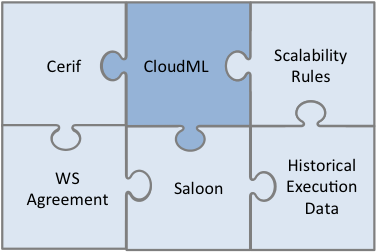
\includegraphics[width=0.6\textwidth,natwidth=200,natheight=150]{./fig/dsl.png}
	\centering
	\label{fig:dsls}
\end{figure}

The Social Network Platform that this thesis proposes is part of the PaaSage EU Project~\cite{paasage}.
The PaaSage perspective is to be a tool for a cloud deployment Specialist to leverage the complex task of deploying an application to the clouds. Usually, a cloud deployment specialist could easily learn the interface and features of one Cloud provider, but it would be very costly and time consuming to leverage the development to many providers. It is a real challenge to orchestrate the simultaneous deployment to many different Clouds at the same time. The main objective of PaaSage is to assist the developer to deal with difficult deployment scenarios through automatic cloud deployment. In order to satisfy this, several components are included to the PaaSage ecosystem. The Profiler components read the CAMEL models and convert them into a constraint programming model by defining the variables of the model, their domains, and the constraints that must be satisfied by the deployment. Also, the Profiler checks all constraints of the CAMEL model and sets the domains of the variables accordingly. The reasoning component analyses the model and finds how deployment candidates should be evaluated. Once a solution has been found, the reasoning component converts the model to Cloud Provider Specific Models (CPSM) for the providers involved in the proposed deployment. The adapter component takes the CPSMs, produces and validates a configuration plan, and sends this plan to the execution ware. The execution ware~\cite{baur2014towards} receives the deployment plan from the adapter and enacts the deployment of the application on the selected providers. Furthermore, the execution ware interacts with the Cloud providers, acquires the virtual machines, configures them and launches the user application on the set of virtual machines. Once the machines are running, the execution ware collects sensor data for the running application, triggering re-configurations if necessary.

The Social Network Platform brings to the DevOps users a friendly interface to browse, discover, view and discuss Application Models. Furthermore, it presents a way to deploy and run these Application Models, by using the previously mentioned components under the hood, and mines their execution history data.

The key contributions of this Social Network Platform(SNP) are the following:
\begin{itemize}
\item The SNP binds all the Social Networking aspects such as friends, new feeds, personal messages etc. with the engineering aspects of creating and deploying application models.
\item The SNP brings the execution histories of the CAMEL applications in the light, providing the end users the ability to browse, discus, point and find essential information needed for other applications.
\item The SNP uses the best known practices both for the front end viewing system and the back end technology.
\item The SNP runs on a horizontal scale architecture with memcached at the back end to reach near real time interaction. 
\end{itemize}



\section{Related Work}
This section describes related work for other professional networks and their caching architecture.

\subsection{Caching data}
Facebook, the largest social network, serves billions of requests per second using memcached~\cite{nishtala2013scaling}. In this magnitude of scale Facebook has several pools of memcached servers (regional pools) along the globe. A single request for a page can produce hundred of requests to the back-end system. Memcached used to store not only key-value from MySQL queries but also pre-computed results from sophisticated algorithms. 
In order to achieve a near real time communication experience to the end user, memcached server have to be efficient, reducing latency. 

The research question in such systems is when a particular key will be invalidated. This problem occurs according to ~\cite{nishtala2013scaling} in two cases: (1) \emph{stale sets} and (2) \emph{thundering herds}. A stale set occurs when a web server sets a value to the memcached that does not reflect the real value of the database. Thundering herds occur when a specific key has a heavy read and write activity in the same time. Stale sets resolved by a N-bit token, bound to specific key, sent from memcached to web server that want to update the key when cache miss occurs. If a delete request received then the request for updating this value from that client is rejected. The thundering herbs solved by configuring memcached servers return a N-bit token only once every ten seconds per key.

Linkedin, the largest professional network, stores hundreds of terabytes of data to Project Voldemord~\cite{sumbaly2012serving}, a key-value store, inspired by Amazon Dynamo~\cite{decandia2007dynamo}. Linkedin stores to Voldemort pre-computed offline data for example results of data mining applications such as features like ``People You May Know'' which running on hundreds of terabytes to make an estimation, using Hadoop as the computational component of those estimations. 
Voldemord compared with Dynamo has the same following requirements: (1) a simple \emph{get/put} application interface (2) A \emph{replication} factor, the number of replicas for each key-value tuble, implemented using vector clock (3) a \emph{required read} factor to succeed a get request, (4) a \emph{required write} factor to succeed a put request. 

\subsection{Professional Networks}

%During the last few years social networking has evolved into a fundamental daily activity for many individuals and a new frontier for business marketing. Besides “traditional” social networking, a recent trend is professional and domain-specific networking services focused on interactions and relationships of a business nature around a specific target domain. These online communities have the potential to become a platform for collective intelligence and open innovation~\cite{leimeister2010}, a medium for knowledge-centered collaboration~\cite{faraj2011}, and a trustworthy decision-support tool~\cite{bulmer2010}.
 
IT professionals use a variety of online sources as aids in their daily tasks. Developers typically prefer community-moderated forums over vendor-moderated sites. Social networks focusing on software technology in particular provide developers with the opportunity to leverage the knowledge and expertise of their peers.
 
One of the most popular such platforms is GitHub~\cite{github_url}, a collaborative revision control platform for developers launched in April 2008, and arguably the largest code-hosting site in the world. 
GitHub provides social networking functionality such as feeds, followers, wikis and a social network graph that captures how developers work on versions of their repositories, which version is newest, etc.
Gitter~\cite{gitter} is a related service that facilitates discussions between members of GitHub communities by providing a long-term chat integrated with code and issues.
Sourceforge~\cite{sourceforge} was the first code-hosting platform offered to open-source projects. It was launched in 1999 and offered IT professionals the ability to develop, download, review, and publish open-source software. Sourceforge is similar to GitHub in its support for social features.
Other similar code-hosting platforms are Google Code~\cite{googlecode} and Microsoft CodePlex~\cite{codeplex}.
None of those platforms collect, analyze, or use information from executions of application deployments to improve the level of technical discussion between users or abstract code structure through modelling or enhance user interactions through the use of analytics over application execution histories.

StackOverflow~\cite{stackoverflow} advances on earlier Q\&A sites in which users ask and answer questions. Users can vote up or down questions and answers and earn \emph{reputation points} and \emph{badges} in return for their active participation. 
Although StackOverflow and GitHub address different aspects of software development (StackOverflow is not a code-hosting platform) there is a synergy and correlation between the two~\cite{stackgit}. The proposed social network platform extends StackOverflow through the use of social networking features that enable users interested in reasoning about application deployments to use and share knowledge drawn from analyses of information repositories.
 
IBM's BlueMix~\cite{Bluemix-dev} is a development and support platform for communities of DevOps users wishing to compose distributed applications out of components drawn from libraries and deploy them at IBM-provided and supported cloud infrastructure.  BlueMix is a key component of IBM's DevOps best practices~\cite{ibm-devops} for achieving rapid prototyping, automated deployment, and continuous testing of software. BlueMix encourages its users to ask their questions to StackOverflow but also includes a community forum~\cite{Bluemix-dev} with rating of answers contributes to eventually building a basic knowledge base, similar to traditional approaches such as StackOverflow.  The proposed social network platform system differs from BlueMix in its support for expressing applications as models (CloudML, CAMEL) and its use of two information repositories, the PaaSage repository of models and execution histories and Chef supermarket, and the use of analytics over past executions to enable users to reason about application deployments. A common feature between the proposed social network platform and BlueMix is support for deployment of distributed applications. 

LinkedIn widely adopted across a range of professional communities due to its robust set of social features (and to some extent due to its use of extensive analytics over collected information~\cite{sumbaly2013big}), LinkedIn provides no specific support for software engineering activities and thus more closely resembles traditional social networking platforms such as Facebook.


The lack of Social Networking features of github came to fill the Geeklist platform~\cite{geeklist_url}, where developers and IT companies can discover and share the work they have done, connect with other companies with a social network manner or join development communities. Another code hosting platform is Snipplr ~\cite{Snipplr_url}, where developers can upload short code snippets and not full programs in order to keep all of their frequently used code in one place that's accessible from any computer and any user. Masterbranch~\cite{masterbranch_url} is a new under development platform that allows collating and sharing of projects within user profile. Profile works similarly to LinkedIn and has an incentivisation scheme called DevScore coupled with unlockable achievements in adds gamification element. Dzone~\cite{dzone_url} is essentially a link repository for developers allowing link sharing and incentivisation based around voting for popular links. The Code project~\cite{codeproject_url} website and forum allows code-specific discussion and shares relevant articles and news, contains blogs,  newsletter and has a questions and answers section.

The above systems can be further classified based on whether they use a repository to store software-related information (code, models, configuration, or execution histories) and whether this information is shared and raised through crowd sourcing~\cite{	howe2006rise}.  GitHub, GoogleCode, CodePlex, SourceForge, BlueMix, Chef Supermarket, and our platform store at least one type of software-related information and all systems but BlueMix are raising shared content in their software-related repositories via crowd sourcing. Our professional network is the only solution that analyzes information in its software-related repositories to assist users with suggestions and hints. 



\begin{table*}[h]

\begin{threeparttable}

\caption{Feature comparison.}
\label{tab:related}


\begin{tabular}{c|c|c|c|c|c|c|c|c|c|cc}

\cline{2-10}
  &  \multicolumn{4}{c|}{User Interaction} & \multicolumn{5}{c|}{Repository} &  &  \\ 
\cline{2-12} 
  &
   
  \begin{tabular}[c]{@{}c@{}}\rot{Social features \tnote{a}} \end{tabular} & 
  \begin{tabular}[c]{@{}c@{}}\rot{Groups} \end{tabular} &
  \begin{tabular}[c]{@{}c@{}}\rot{Q \& A} \end{tabular} &
  \begin{tabular}[c]{@{}c@{}}\rot{Personal  messaging} \end{tabular} & 
  \begin{tabular}[c]{@{}c@{}}\rot{Software code}\end{tabular} & 
  \begin{tabular}[c]{@{}c@{}}\rot{Software models}\end{tabular} & 
  \begin{tabular}[c]{@{}c@{}}\rot{Software config}\end{tabular} & 
  \begin{tabular}[c]{@{}c@{}}\rot{Execution histories}\end{tabular} & 
  \begin{tabular}[c]{@{}c@{}}\rot{Crowd sourced}\end{tabular} & 
  \multicolumn{1}{c|}{\begin{tabular}[c]{@{}c@{}}Repo\\ assisted\\ hints \tnote{b} \end{tabular}} & 
  \multicolumn{1}{c|}{\begin{tabular}[c]{@{}c@{}}Application\\ deployment\end{tabular}} \\ 
\hline

\multicolumn{1}{|c|}{GitHub} & \cmark & \xmark & \xmark & \xmark & \cmark & \xmark & \xmark & \xmark & \cmark & \multicolumn{1}{c|}{\xmark} & \multicolumn{1}{c|}{\xmark} \\
\hline
\multicolumn{1}{|c|}{Sourceforge} & \cmark & \xmark & \cmark & \cmark & \cmark & \xmark & \xmark & \xmark & \cmark & \multicolumn{1}{c|}{\xmark} & \multicolumn{1}{c|}{\xmark} \\
\hline
\multicolumn{1}{|c|}{GoogleCode} & \xmark & \xmark & \cmark & \xmark & \cmark & \xmark & \xmark & \xmark & \cmark & \multicolumn{1}{c|}{\xmark} & \multicolumn{1}{c|}{\xmark} \\
\hline
\multicolumn{1}{|c|}{CodePlex} & \cmark & \xmark & \cmark & \cmark & \cmark & \xmark & \xmark & \xmark & \cmark & \multicolumn{1}{c|}{\xmark} & \multicolumn{1}{c|}{\xmark} \\
\hline
\multicolumn{1}{|c|}{StackOverflow} & \xmark & \xmark & \cmark & \xmark & \xmark & \xmark & \xmark & \xmark & \xmark & \multicolumn{1}{c|}{\xmark} & \multicolumn{1}{c|}{\xmark} \\ 
\hline
\multicolumn{1}{|c|}{BlueMix} & \xmark & \xmark & \cmark & \xmark & \xmark & \xmark & \cmark & \xmark & \xmark & \multicolumn{1}{c|}{\xmark} & \multicolumn{1}{c|}{\cmark} \\ 
\hline
\multicolumn{1}{|c|}{Chef Supermarket} & \xmark & \xmark & \xmark & \xmark & \xmark & \xmark & \cmark & \xmark & \cmark & \multicolumn{1}{c|}{\xmark} & \multicolumn{1}{c|}{\xmark} \\ 
\hline
\multicolumn{1}{|c|}{LinkedIn} & \cmark & \cmark & \cmark & \cmark & \xmark & \xmark & \xmark & \xmark & \xmark & \multicolumn{1}{c|}{\xmark} & \multicolumn{1}{c|}{\xmark} \\ 
\hline
\multicolumn{1}{|c|}{geeklist} & \cmark & \cmark & \xmark & \xmark & \xmark & \xmark & \xmark & \xmark &  & \multicolumn{1}{c|}{ \xmark } & \multicolumn{1}{c|}{ \xmark } \\
\hline
\multicolumn{1}{|c|}{Snipplr} & \xmark & \xmark & \xmark & \xmark & \cmark & \xmark & \xmark & \xmark &  & \multicolumn{1}{c|}{\xmark} & \multicolumn{1}{c|}{\xmark} \\ 
\hline
\multicolumn{1}{|c|}{Masterbranch} & \xmark & \xmark & \xmark & \xmark & \cmark & \xmark & \xmark & \xmark &  & \multicolumn{1}{c|}{\xmark} & \multicolumn{1}{c|}{\xmark} \\ 
\hline
\multicolumn{1}{|c|}{Dzone} & \cmark & \xmark & \xmark & \xmark & \cmark & \xmark & \xmark & \xmark &  & \multicolumn{1}{c|}{ \xmark} & \multicolumn{1}{c|}{\xmark } \\ 
\hline
\multicolumn{1}{|c|}{codeproject} & \cmark & \xmark & \cmark & \xmark & \cmark & \xmark & \xmark & \xmark &  & \multicolumn{1}{c|}{\xmark} & \multicolumn{1}{c|}{\xmark} \\
\hline
\hline
\multicolumn{1}{|c|}{PaaSage SN} & \cmark & \cmark & \cmark & \cmark & \xmark & \cmark & \cmark & \cmark & \cmark & \multicolumn{1}{c|}{\cmark} & \multicolumn{1}{c|}{\cmark} \\ 
\hline

\end{tabular}

\begin{tablenotes}
      \small
       \item[a] Features: follow and news feed
      \item[b] User assistance based on data analysis of the repository
\end{tablenotes}
\end{threeparttable}
\end{table*}

\chapter{Management of ...}

General discussion \ldots

\section{AA}

\section{BB}

\section{CC}

\section{DD}

\chapter{Implementation}
\label{chap:implementation}
This chapter describes the implementation of our social networking site, the User Interface and how the system scales.

The system architecture is consisting of the following components, as shown in Figure~\ref{fig:system_architecture}: 
\begin{itemize}
\item In the first layer, which is the front-end layer, lives (1) the social networking engine, which runs all the PHP scripts, as described in Section~\ref{sec:implementaion_of_social_netowrk} and (2) the CDO client which is responsible for the communication with the repository of the application models, as described in Section~\ref{sec:cdo_comm}. 
\item In the second layer, which is the caching layer, lives the Memcached caching system, which described in Section~\ref{sec:memcache_implementation}. 
\item In the third layer, which is the back-end of the system, lives the social network MySQL database, the CDO server, as well as the CDO repository of application models, which is a MySQL database. 

\end{itemize}
\begin{figure}[h]
	\centering
	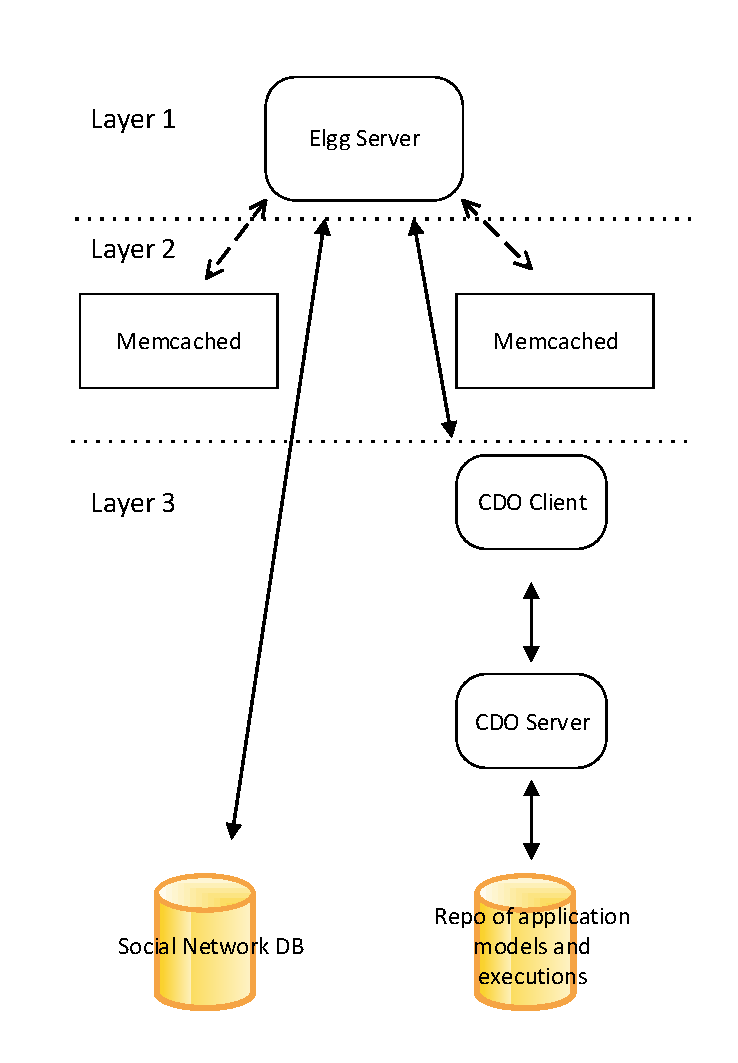
\includegraphics[width=0.9\textwidth,natwidth=200,natheight=150]{./fig/system_architecture.pdf}
	\caption{The overall social networking architecture}
	\label{fig:system_architecture}
\end{figure}

In order to achieve the scalability of the system, two different system architectures are examined at the first two layers: (1) We added more than one social network engines at the first layer of the system. In this implementation, in order to keep the file system in consistent mode we integrated NFS server along with Apache Zookeeper~\cite{zookeeper_url} as described in Section~\ref{sec:engine_scale}. (2) We added more than one memcached nodes at the second layer in order to add more CPU capacity and improve the system's response time.

\section{Social networking platform}
\label{sec:implementaion_of_social_netowrk}
The social networking platform is implemented over the extensible Elgg social network framework~\cite{elgg_url}.  Elgg is an open source software written in PHP, that uses MySQL for data persistence and supports jQuery~\cite{jquery_url} for client-side scripting.  

The overall architecture of Elgg Social Network is shown in Figure~\ref{fig:elgg_architecture}. The Elgg Social Network is structured following the key concepts of Model - View - Controller (MVC) known architectural pattern for User Interfaces. The MVC system is analyzed here, depicting the most important aspects of it from the Elgg's perspective. Explaining the Elgg's architecture by using MVC system will make the understanding of Elgg less complex.

Figure~\ref{fig:elgg_architecture} shows the model, view, and controller parts of Elgg's architecture. In a typical scenario, a web client requests an HTML page (e.g., the description of an application model).  The request arrives at the \emph{Controller}, which confirms that the application exists and instructs \emph{Model} to increase the view counter on the application model object. The controller dispatches the request to the appropriate handler (e.g., application model, component handler, community handler) which then turns the request to the view system. View pulls the information about the application model and creates the HTML page that is returned to the web client.

The {\bf Model} of the framework is structured around the following key concepts as shown in Figure ~\ref{fig:elgg_entities}:
\begin{itemize}
\item \emph{Entities}, classes capturing social networking concepts: users, communities, application models. Elgg Core comes with four basic objects: ElggObject, ElggUser, ElggGroup, ElggSite, ElggSession, ElggCache and a lot of other classes necessary for the proper engine operation.
\item \emph{Metadata} describing and extending entities (e.g., a response to a question, a review of an application model, etc.).
\item  \emph{Relationships} connect two entities (e.g., user A is a friend of user B, user C is a contributor to an application model, etc.) and are persisted in the social network database.
\item \emph{Annotations} are pieces of simple data attached to an entity that allow users to leave ratings, or other relevant feedback.
\end{itemize}

\begin{figure}[h]
	\centering
	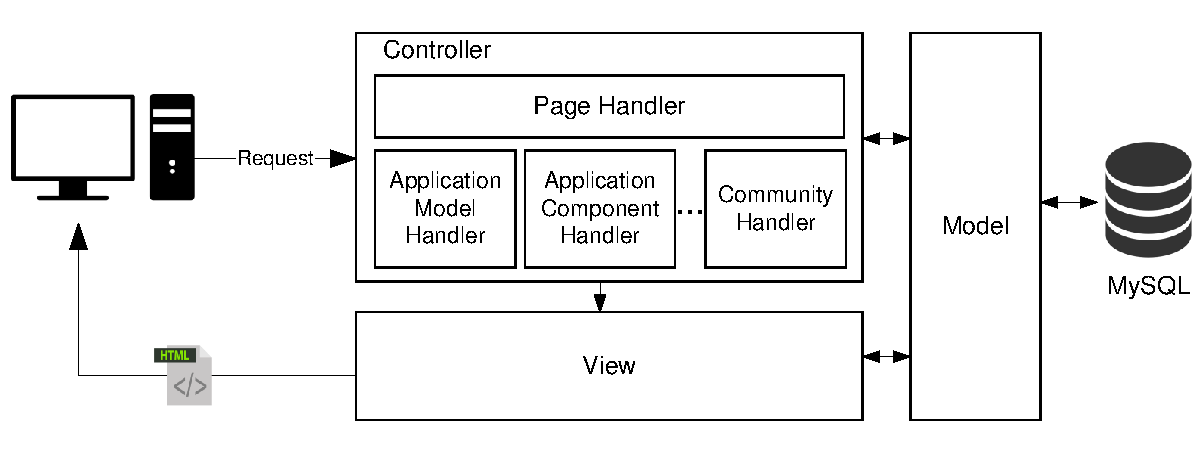
\includegraphics[width=0.9\textwidth,natwidth=200,natheight=150]{./fig/elgg_architecture.pdf}
	\caption{Architecture of the Elgg social networking engine}
	\label{fig:elgg_architecture}
\end{figure}

All Elgg objects inherit from ElggEntity, which provides the general attributes of an object. Elgg core comes with the following basic entities: ElggObject, ElggUser, ElggGroup, ElggSite, ElggSession, ElggCache, as well as other classes necessary for the operation of the engine.

\begin{figure}[h]
	\centering
	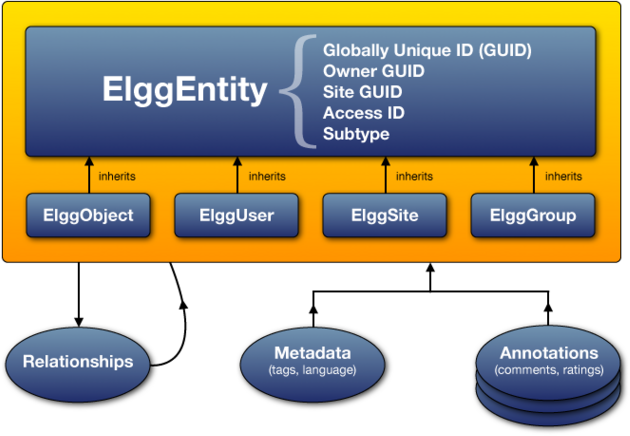
\includegraphics[width=0.6\textwidth,natwidth=200,natheight=150]{./fig/elgg_data_model.png}
	\caption{The Elgg engine data model}
	\label{fig:elgg_entities}
\end{figure}

The {\bf controller} component of MVC model of Elgg consisting of the \emph{Actions} of the system which are the primary way the users interact with the Elgg site. An action in Elgg Framework is the code that make changes to the database when a user performs an action like logging in, posting a comment, or creating an application model. The action script processes input, makes the appropriate modifications to the database, and provides feedback to the user about the action. By default, actions are only available to logged in users and include Cross-Site Request Forgery (CSRF) Security token to overcome session fixation~\cite{kolvsek2002session}, Session Hijacking~\cite{burgersposter} and Cross-site Scripting~\cite{thamescomparing}.

Additionally, the controller component includes the \emph{Events} and the \emph{Plugin Hooks}, which are used in Elgg Plugins to interact with the Elgg engine. Events and hooks are triggered at important times throughout Elgg’s boot and execution process, and allows plugins to modify or cancel the default behaviour of Elgg. When an event is triggered, a set of handlers is executed in order of priority. Each handler passes the arguments and has the option to influence the process. When the execution of the current handler is completed, the ``trigger'' function returns a value based on the behaviour of the handlers.

The {\bf View} component is responsible for creating the output. Generally, this will be HTML sent to a web browser, but it could also be XML, JSON or any other data formats. View handles everything from the layout of pages and chunks of presentation output (like a topbar ) down to individual links and form inputs.

Elgg comprises a core system that can be extended through plugins (examples are the Cart system and the handling of Application Models). Plugins add new functionality, can customize aspects of the Elgg engine, or change the representation of pages.
A plugin can create new objects (e.g., ApplicationObject) characterized (through inheritance of ElggEntity) by a numeric globally unique identifier (GUID), an owner GUID and an Access ID. Access ID encodes permissions ensuring that when a page requests data it will not touch any data the current user does not have permissions on. All plug-ins share a common structure of folders and PHP files, following the MVC model of Figure~\ref{fig:elgg_architecture}.  

The hierarchy of a plug-in is shown in Figure~\ref{fig:elgg_hierarchy}. 
The folder {\em actions} includes the actions applied on application models. Every active participation of the user is performed via an action. Logging in, creating, updating or deleting content are all general categories of actions.
The {\em views} folder contains the {\em php} forms applied on application models, {\em river} events (Elgg terminology for live feeds). Viewss are responsible for creating the output for the client browser. Generally, this will be HTML, but it can be also JSON or other format. 
{\em Pages} overrides elements of core Elgg pages and can be from chunks of presentation output (like sidebars) down to individual html code.  
The {\em js} and {\em lib} folder provides javascript and {\em php} library functions. 
Finally, the {\em vendors} folders include third-party frameworks such as Twitter's bootstrap front-end~\cite{bootstrap_url}.
The most important file of a plug-in is the \emph{start.php} script, which contains the \emph{page handler}. Page handler is a function manages the plug-in pages enabling custom url redirect to a specific page. 
The plug-in initialization is also defined in the start.php and registers actions, events and determines the views. 

\begin{figure}[h]
	\centering
	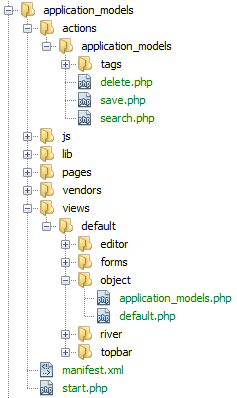
\includegraphics[width=0.4\textwidth]{./fig/folder_hierarchy.png}
	\caption{The structure of the application description plug-in}
	\label{fig:elgg_hierarchy}
\end{figure}

Finally, as mentioned before, for client side scripting the jQuery is used. The main reason why jQuery is preferred in this work over of pure JavaScript~\cite{mccormick2004jquery} is that it's a light library which pushes content to the client machine, it therefore reduces the wait time for server response. Plus, it's smaller than Flash, so it results in smoother playbacks and less errors. Furthermore, jQuery works anywhere since is cross-browser compatible with any browser, mobile phone or tablet, and Apple devices. Finally, another hand-solving advantage of jQuery is its simple syntax.It is designed to make it easier to navigate in a document, select HTML DOM elements, create animations, handle events, and developing Ajax applications. 

Thus, the jQuery is used by SNP for implementing client side scripting and for the remaining of this chapter, when we refer to JavaScript, we actually refer to the jQuery library. 
Furthermore, some other JavaScript libraries are used in order to make the User Interface more powerful. One of those libraries is the Chart.js~\cite{chartjs_url} library which is used to generate the graphs and charts in execution's page.

\subsection{Extending the core Elgg platform}
As described in the previous section, the new functionality of Elgg social networking platform can be introduced by new plugins. Since the modification of the core system is not a good practice, because it makes the system more difficult to implement and does not let it upgrade to the new versions of Elgg framework. The following plugins are implemented:

\textbf{ApplicationModel}. The ApplicationModel plugin has a {\it page handler} to manage the application Model pages. Also, ApplicationModel has client side JavaScript for manipulating User Interaction and dynamic pages. Furthermore, some php libraries are implemented, for example a library for interaction with CDO client or a library for manipulating Application models. 

\textbf{Components}. The Components plugin has a {\it page handler} to manage the Components pages and their Categories and a PHP library to interact with Chef supermarket.

\textbf{CustomView}. The CustomView plugin has all the necessary customization of the PaaSage social networking platform (PSNP). All custom views of the system are implemented in this plugin. This plugin overrides all the default views of the Elgg that should be changed and contains client side JavaScript. Furthermore, CustomView has the following seven page handlers: {\t profile} responsible for profile pages, {\t avatar} responsible for the photos of user pages, {\t settings} responsible for the pages of user settings, {\t friends} responsible for the friends of the user pages, {\t contact} responsible for the Contact Information of the PSNP, {\t review} responsible for the reviews of Application Models and {\t search} responsible for the main search facility of PSNP. Finally, CustomView has all the required \emph{Actions} of the plugin such as the vote up or down, the action to add a review etc.

\textbf{NotificationSystem}. This plugin is responsible for the notifications of the Social Network which contains a relevant page handler, JavaScript for client side scripting and a php server side library.

\textbf{Tags}. This plugin does not include any page handlers but only the necessary actions for the Tags such as {\it add} or {\it delete} a Tag and a php library responsible for those. 

\textbf{UserStatistics}. This plugin is responsible for collecting and displaying the information about the Users.

\textbf{Memcached}. This plugin has all the essential functionality for memcached implementation as will be described in Section~\ref{sec:memcache_implementation}.

\textbf{ZookeeperRecipes}. This plugin has all the essential functionality for memcached implementation as will be described in Section~\ref{sec:engine_scale}.

\textbf{Groups}. The Groups plugin is the default plugin of Elgg Framework modified to support the required functionality.

\textbf{Messages}. The Messages plugin is the default plugin of Elgg Framework modified to support the required functionality.

\subsubsection{Twitter bootstraping of Elgg}
Responsive web design (RWD)~\cite{natda2013responsive} is a web design approach aiming at crafting web application sites to provide an optimal viewing experience, which it provides easy reading and navigation with a minimum of resizing, panning, and scrolling, across a wide range of devices (from mobile phones to desktop computer monitors). However, the default CSS of Elgg, which is part of the View component of architecture, does not offer responsive web pages. Thus the ideal solution is to integrate Twitter Bootstrap to Elgg viewing system. 

Twitter Bootstrap~\cite{twitter_bootstrap}~\cite{cochran2012twitter} is a free and open-source collection of tools for creating dynamic websites and web applications. It contains HTML and CSS-based design templates for typography, forms, buttons, navigation and other interface components, as well as optional JavaScript extensions. It aims to ease the development of dynamic websites and web applications. 

We customize the Elgg view inserting the Twitter Bootstrap view system. The default view system of Elgg changed to support the Twitter Bootstrap responsive grid.

\subsection{Communicating with CDO server}
\label{sec:cdo_comm}
As mentioned in~\ref{sec:background}, the execution history of deployments of application models and the description of those models are stored in the CAMEL information repository, which is implemented as an Eclipse CDO server. In order to communicate with the CDO server, a CDO Java client is needed. The CDO client stands between the social networking engine (Elgg server) and the CDO server, making the exchange of information between those two possible, as shown in Figure~\ref{fig:system_architecture}.

Specifically, regarding the communication between the CDO server and the client, the CDO client opens one or more sessions to the CDO server. Each session represents a connection to the CDO repository and provides a broad API to interact with it. A session does not provide direct access to model instances; views or transactions are needed in order to navigate or modify the model instance graph. The implemented CDO client exposes read/write access to the repository for either viewing the execution histories or the model of the applications, or for storing new execution models. For the communication between the social networking engine and the CDO client, the CDO client exposes a RESTful API to the social networking engine providing all the necessary methods. 

For example, when a user from the social network platform requests the execution histories of an application, the engine sends a request to the CDO client through the RESTful API, the CDO client receives the request and forwards an appropriate request to the CDO server. The CDO server receives the request and queries the repository of application models and executions. When the CDO server receives the response, it forwards the response back to the CDO client, which forwards the response back to the social networking engine. The social networking engine transforms the response to JSON format, in order for it to be readable by the JavaScript. JavaScript plays the final role, by projecting the execution histories in a proper table to the end user that requested the page of the executions of an application.

As a future work, message queue techniques can be used for the communication between the CDO client and the social networking engine. One message queue technique is ZeroMQ~\cite{zeromq_url} which is a high-performance asynchronous messaging library, aimed at use in scalable distributed applications. Another well-known message queue system is RabbitMQ~\cite{rabbitmq_url}, which is a messaging broker and provides a common platform to send and receive messages. Those techniques achieve communication between different language components of an application.

\section{Scalability}
A lot of work has been made on the scalability of social networking platforms. The scale of social networks is very important for platforms such as Facebook which has one billion users. We integrate known practises to make the social networking platform scalable and efficient. From where the Elgg social networking engine was implemented to run in only one single machine, in this work, we distribute and design a scalable architecture. We replicated the social networking engine and we introduced caching techniques into our architecture.

\subsection{Social networking engine}
\label{sec:engine_scale}
This section describes how the horizontal scale of social network engine is achieved by adding more than one Elgg servers. At the layer 1 of Figure~\ref{fig:elgg_architecture} lives the Apache2 server, which as the stress test of the system indicates in Chapter~\ref{chapt:evaluation}, takes a heavy load on CPU utilization. 

The heavy load of Apache2 server occurs by the nature of Elgg framework. Because the Elgg core system is implemented to be extensible and configurable, every time a simple page or just an AJAX call is received by the Elgg, the Elgg framework performs the following heavy tasks: it broadcasts an {\it init system} event; this event is caught by all plugins of Elgg and at this initialization phase the plugins register: (1) the page handlers, (2) the PHP libraries, (3) the actions, (4) the events and hooks, (5) the JavaScript libraries and (6) the CSS scripts. Therefore, all those actions generate a heavy load resulting in consuming CPU utilization and slowing the response time of the system. We introduce more than one Apache2 servers running the social networking engine of Elgg framework to overcome this.  

The social networking engine keeps some information in the file system instead of in the social network database. This information includes the profile photos of users and any other images such as photos that users add to the community groups. Furthermore, the initial configuration of social networking engine keeps in the file system some caching files. Those files represent some views of the web pages which are independent of any specific users and remain unchanged among all users. This file system caching feature is removed from the social network engine because it is more efficient to use memcached for the caching instead of the slow file system.

In order to all social networking engines have access to the same file system, the Network File System (NFS)~\cite{sahni2015network} is used. NFS allows a server to share directories and files with clients over a network. With NFS, users and programs can access files on remote systems as if they were stored locally.

In our implementation, NFS is configured and used in order to allow all social networking engines to gain access to the same file system store. An NFS server is installed in one of the SN engines and all the other SN engines have an NFS client accessing the remote file system.   

Distributing social network engine was not an easy problem to solve, so Apache ZooKeeper~\cite{zookeeper_url} is used in order to achieve synchronization. 
Apache ZooKeeper~\cite{hunt2010zookeeper} is a service for coordinating processes of distributed applications. Since
ZooKeeper is a part of a critical infrastructure, it aims to provide a simple and high performance kernel
for building more complex coordination primitives at the client. 
We use this service in order to enable highly reliable distributed coordination among the file system and the social networking engine. 
Apache ZooKeeper provides a tree abstraction where every node in that tree (or znode) is a file on which a variety of simple operations can be performed. ZooKeeper orders operations on znodes so that they occur atomically. Therefore there is no need to use complex locking protocols to ensure that only one process can access a znode at a time. The tree represents a hierarchical namespace, so that many distinct distributed systems can use a single ZooKeeper instance without worrying about their files. 

Social networking engine uses Apache ZooKeeper in order to keep the file system consistent, in rare but possible scenarios like two users trying to upload a file to the same group simultaneously. When a social networking engine wants to write a file in file system, it first locks the specific path and after finishing the write operation it releases the lock. Thus, a file can never be corrupted.

For communication between the Apache ZooKeeper and the Elgg framework, the php-zookeeper-recipes~\cite{zookeeper_recipes_url} are used by the ZookeeperRecipes plugin. Specifically, the {\it exclusive locks} of Zookeeper are used to keep the system in consistent mode.

\subsection{Memcached}
\label{sec:memcache_implementation}
This section describes how we integrated memcached~\cite{memcache_url} to our system architecture. Memcached is an open source, high-performance, distributed memory object caching system. We chose memcached, because it is a generic simple in-memory key-value store. It has a powerful API available for PHP. After memcached integration the system decreased its response time and its performance.

Memcached is added in layer 2 of the system architecture as shown in Figure~\ref{fig:system_architecture} and is used for storing the key-value tuples. The following data are stored in memcached: 
\begin{enumerate}
\item MySQL responses, which are values from social network database such as entities of social network engine, applications, components, users, group discussions. By storing those values, there is no need to query the social network database, but SN Engine is getting the key-values directly from memcached.
\item Views of the web pages which are independent of any specific users and remain unchanged among all users, and werte previously were stored in the file system.
\item JavaScript code results. Some JavaScript code is time consuming to be generated. For example, PHP sends the execution data to JavaScript and then it iterates the data in order to generate the tables and the graphs of execution histories.
\item Executions histories from repository of application models. By storing the executions of applications at memcached, the system's response time decreases. That is due to the PHP modules not needing to go through the heavy CDO client-server communication but them getting the executions of applications directly from memcached.
\end{enumerate}

The keys stored in memcached must be unique. This is implemented using as a prefix of the key the globally unique identifier (GUID), generated by Elgg, and a string value which is describing the data. So, the execution data of an application model with QUID 1000 is stored in memcached with key {\it 1000:execution-data} and the value is the json representation of those data. All tuples at memcached are inserted with the maximum key expiration time of thirty days.

\begin{figure}[h]
	\centering
	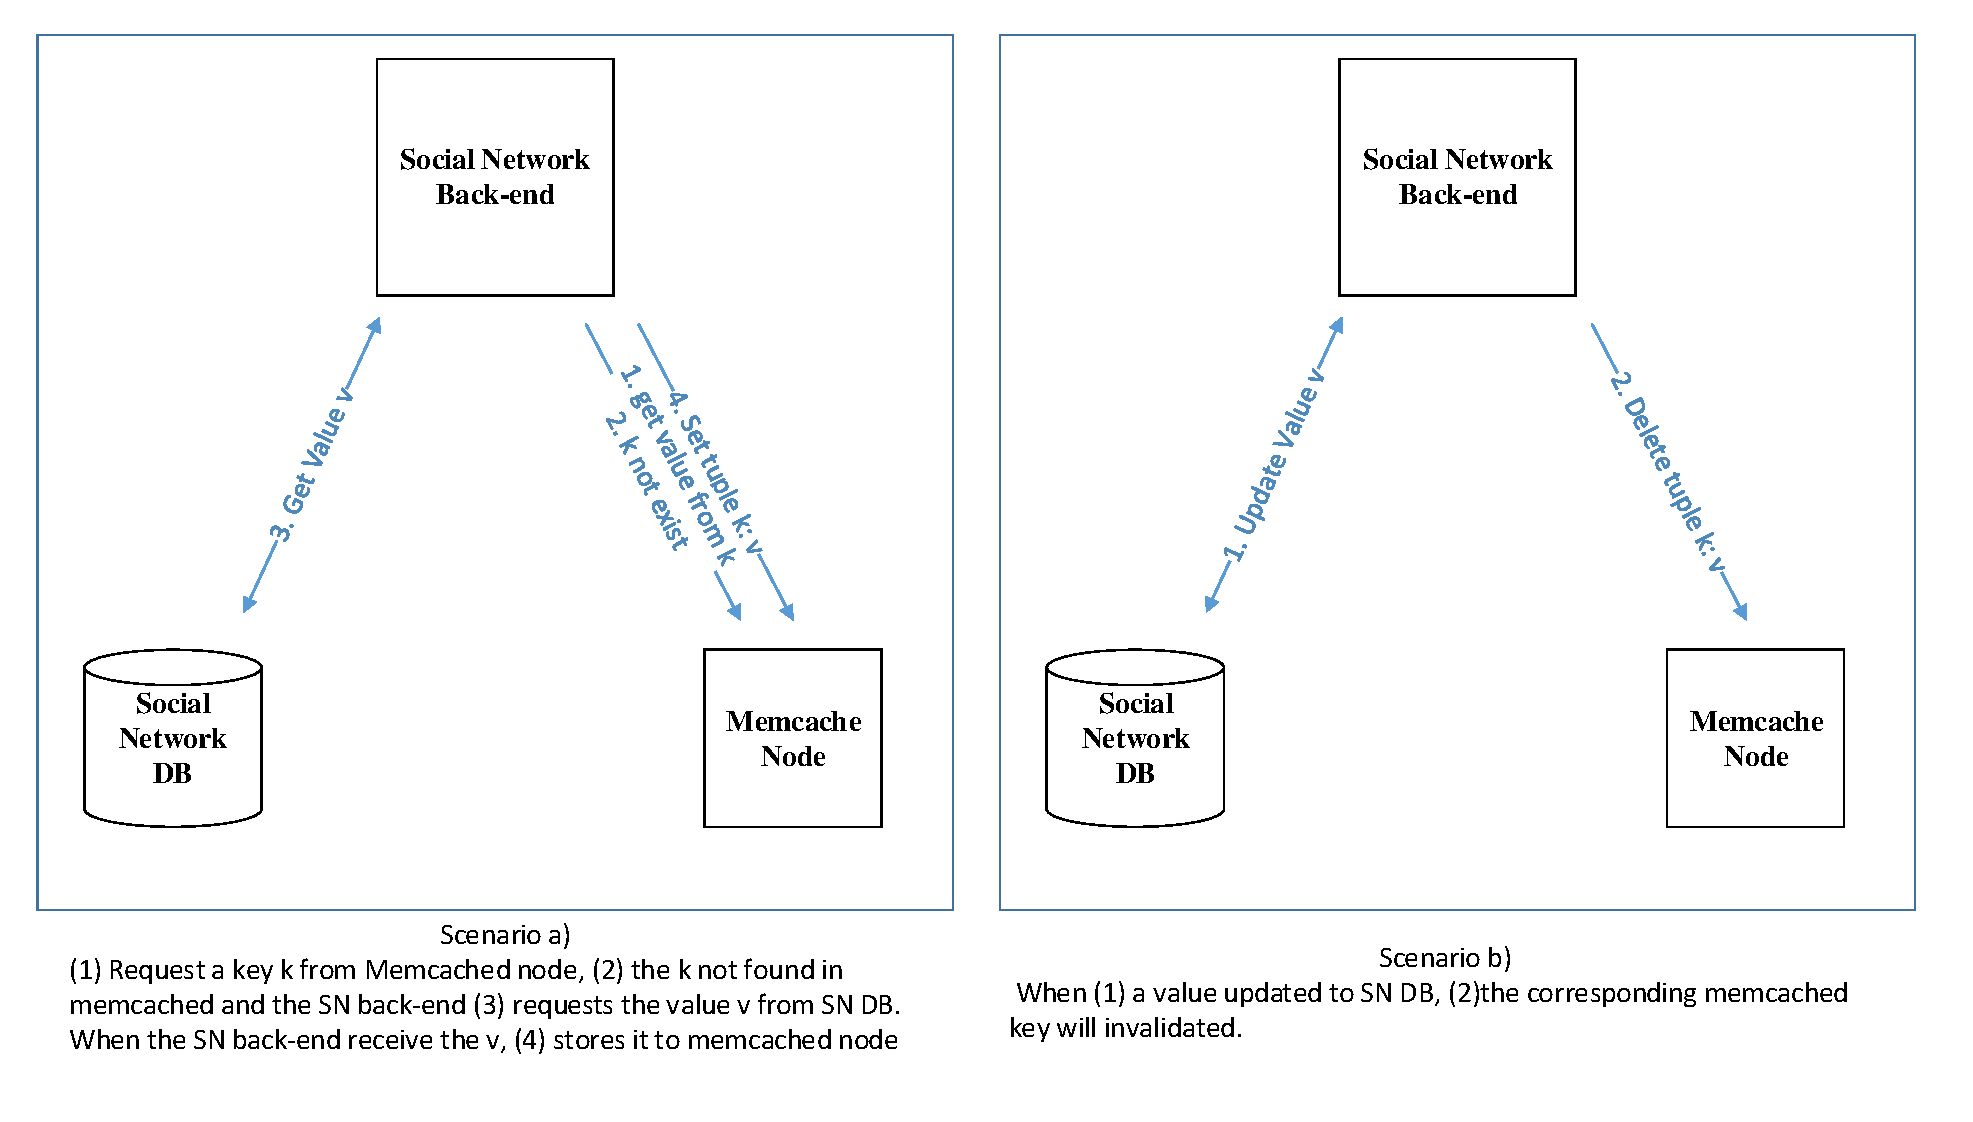
\includegraphics[width=1\textwidth]{./fig/memcached_key_value.pdf}
	\caption{The scenario (a) depicts a request from memcached when the key does not exist and scenario (b) depicts an updated operation of a value}
	\label{fig:memcache_key_value}
\end{figure}

The basic actions of memcached are the get, set and delete of a tuple, as shown in Figure~\ref{fig:memcache_key_value}. In the first scenario, when a value from SNP is requested for a particular key {\it k}, first a query will be send to memcached requesting the tuple with that key {\it k}, if {\it k} not found or it has expired, the SNP will request that key from the social network database. Finally, when SNP gets in touch with the data of the key, it will send those data to be cached in memcached, as shown in the Figure~\ref{fig:memcache_key_value}a. In the other scenario, when a value in the SNP is updated, the memcached key will be deleted(invalidated) as shown in the Figure~\ref{fig:memcache_key_value}b.

The Elgg framework comes with the potential use of memcached but is restricted to the fact that a memcached node must be in the same machine as the Elgg framework. Plus, it makes it more difficult to configure when an insertion in memcached node will take place. Therefore, a new Elgg plugin is implemented called \textbf{Memcached} using the memcached PHP library~\cite{memcached_php_doc}. The basic memcached functions offered by this plugin are: (1) Add memcached nodes, (2) add a key to a node, (3) get a value of a key and (4) delete a key-value item. 

The Apache JMeter~\cite{jmeter_url} was used to measure the response time of the system and the sysstat tool~\cite{sysstat_url} was used to measure the CPU usage. Section~\ref{sec:eval_memcache} 
 shows the performance results of this implementation.

\section{Topic classification}
\label{sec:natural_implementation}
Topic classification, using Natural Language Processing (NLP)~\cite{manning1999foundations}, is a feature added to the social network platform. NLP is used in the interactions between the users and the SNP, in the way the platform can understand and determine the type of user input and provide helpful possible answers.

For example, one real question from the StackOverflow is shown in Figure~\ref{fig:so_question}, which asks the community about the scalability of SQLite and MySQL. From this specific question several important outcomes can be mined. First, this question is very difficult to be answered without using targeted analyses of execution histories of those applications. Second, similar questions can be asked to our own social networking community and would be helpful to use it as a training set to our topic classification tool presented in this section. Finally, many questions of this type exist in the StackOverflow community and we would like to use them in realizing topic classification.

\begin{figure}[h]
	\centering
	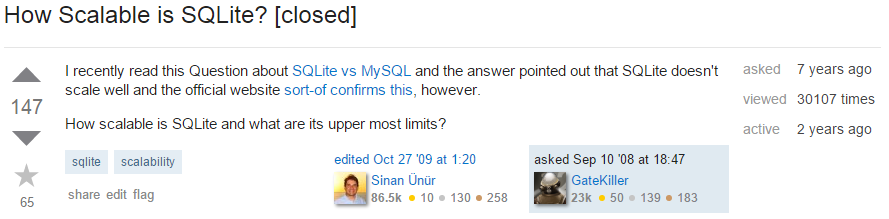
\includegraphics[width=1\textwidth,height=1.65in]{./fig/SOquestion.png}
	\caption{A real example question from StackOverflow}	
	\label{fig:so_question}
\end{figure}

As the Figure~\ref{fig:auto_classification} shows, a user of SNP poses a question to our platform. The platform can process the user's input and classify it into: (1) a similar question that exists in our community or (2) an automatically generated query to the CAMEL repository. In the first scenario, a list of answers from the pre-existing question can be provided as feedback to the new question. In the second scenario, the question can be further processed and a query to CAMEL repository be automatically generated. An automated mechanism can be implement for the second scenario but this is out of the scope of this thesis.  

\begin{figure}[h]
	\centering
	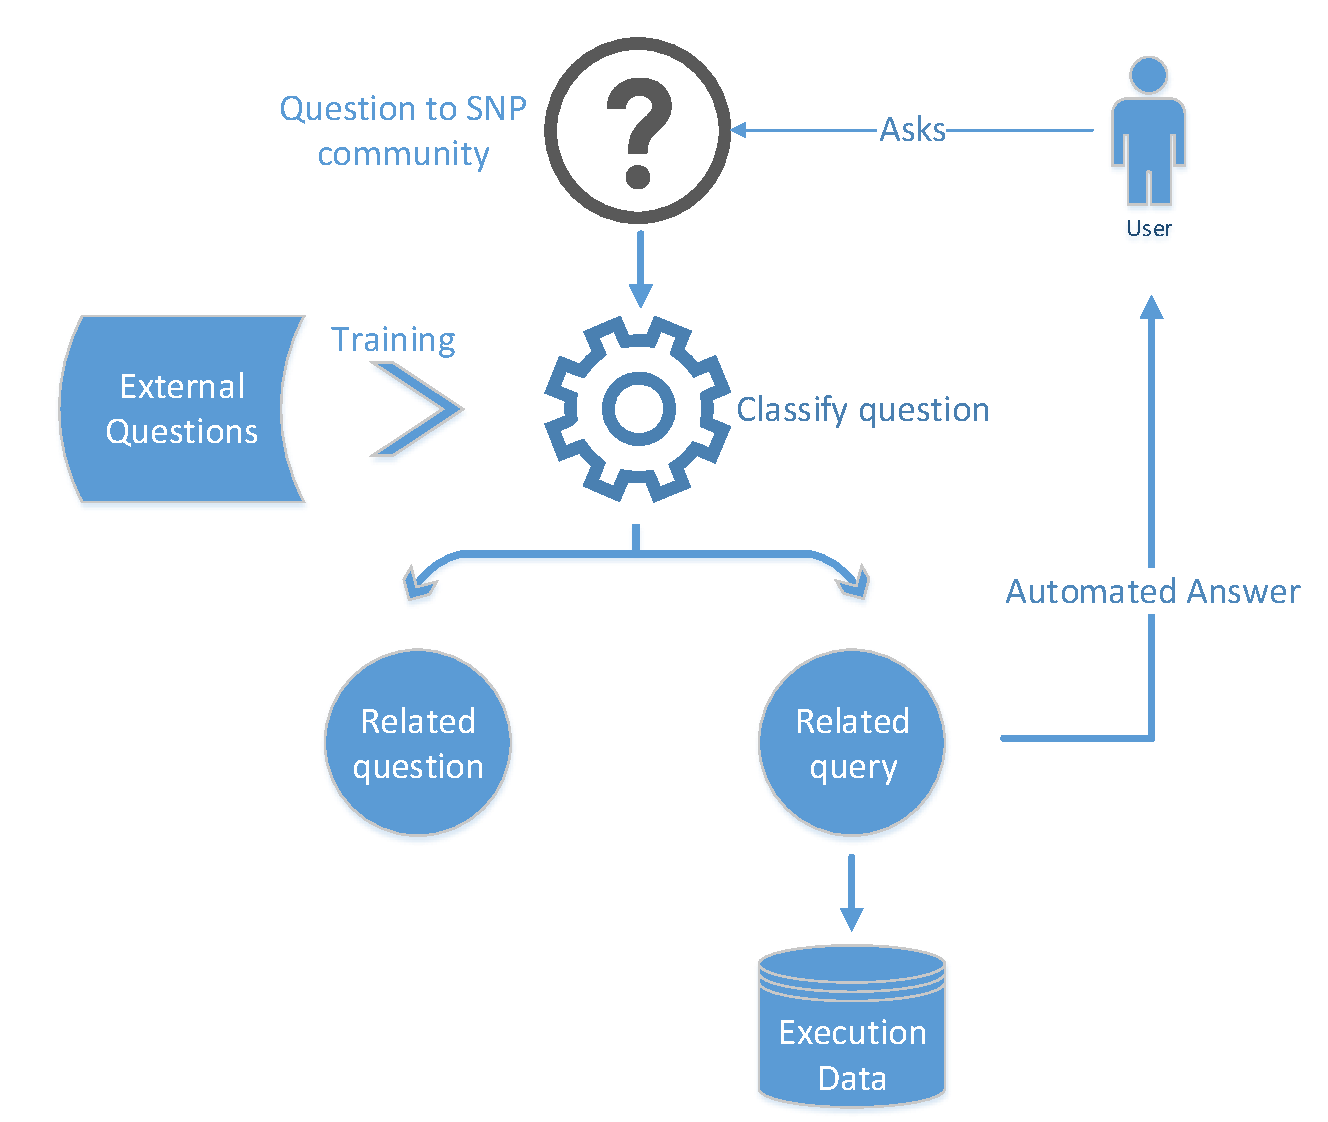
\includegraphics[width=1\textwidth]{./fig/Decision_making.pdf}
	\caption{Classification of questions and automated feedback to user}	
	\label{fig:auto_classification}
\end{figure}

Our implementation lies in between those two scenarios. Some queries to the CAMEL repository are implemented and if a question is asked that in a way resembles a specific query, the platform will provide this query's results as an answer to the user's question. Furthermore, if this question has a similar question and that last question has an answer from a sophisticated user, who had created an hand-crafted query to the repository and had provided the results back to the user, those results can be used as a feedback to the new question. 

We added the Naivy Bayes Natural Language Understanding algorithm to the SN using the Natural framework~\cite{nodenatural_url}, which is implemented with node.js. In general, machine learning algorithms such as Naivy Bayes require an input of training data, called data set. This training data is pulled from questions users post in StackOverflow (SO). Those questions are an excellent repository to train the NB algorithm, because they are categorised by tags (this helps our classifier) and are real questions that our social network community may be interested. This was also a necessity since by the time that this implementation took place, the social network platform did not include a sufficiently large amount of questions in its repository.

In general, the main actions that SO users is shown in Figure~\ref{fig:stackoverflow_questions}. When users ask questions in SO, they must specify some tags describing their questions. A tag is a keyword or a label that places their question in a category with other, similar questions. SO users usually try to add as many tags as possible in order to make their questions popular and get them answered. SO permits users to add up to only five tags in each of their questions. After a question is posed, the whole community of SO can vote the question up or down and the privileged users can flag the question as \emph{duplicate}, \emph{off-topic}, \emph{unclear}, \emph{too broad} or \emph{primarily opinion-based}. This way, low quality questions will be removed from the site resulting in keeping the questions repository clear and helpful for other potential developers to use.

For the training sets, the data to train the NB algorithm, the most voted questions of the SO community are used. Those questions have emerged as the best questions in their field and surely, we avoid the case of using a training set with miss-tagged questions that would result a miss-guided NLP classification. The NLP training set is retrieved from SO site using the stack exchange(SE) API~\cite{stackexchange_url}. The SE API is a powerful API, which allows us to take the questions, the answers, the users and all the information that exists in SO site through a programming interface.

\begin{figure}[h]
	\centering
	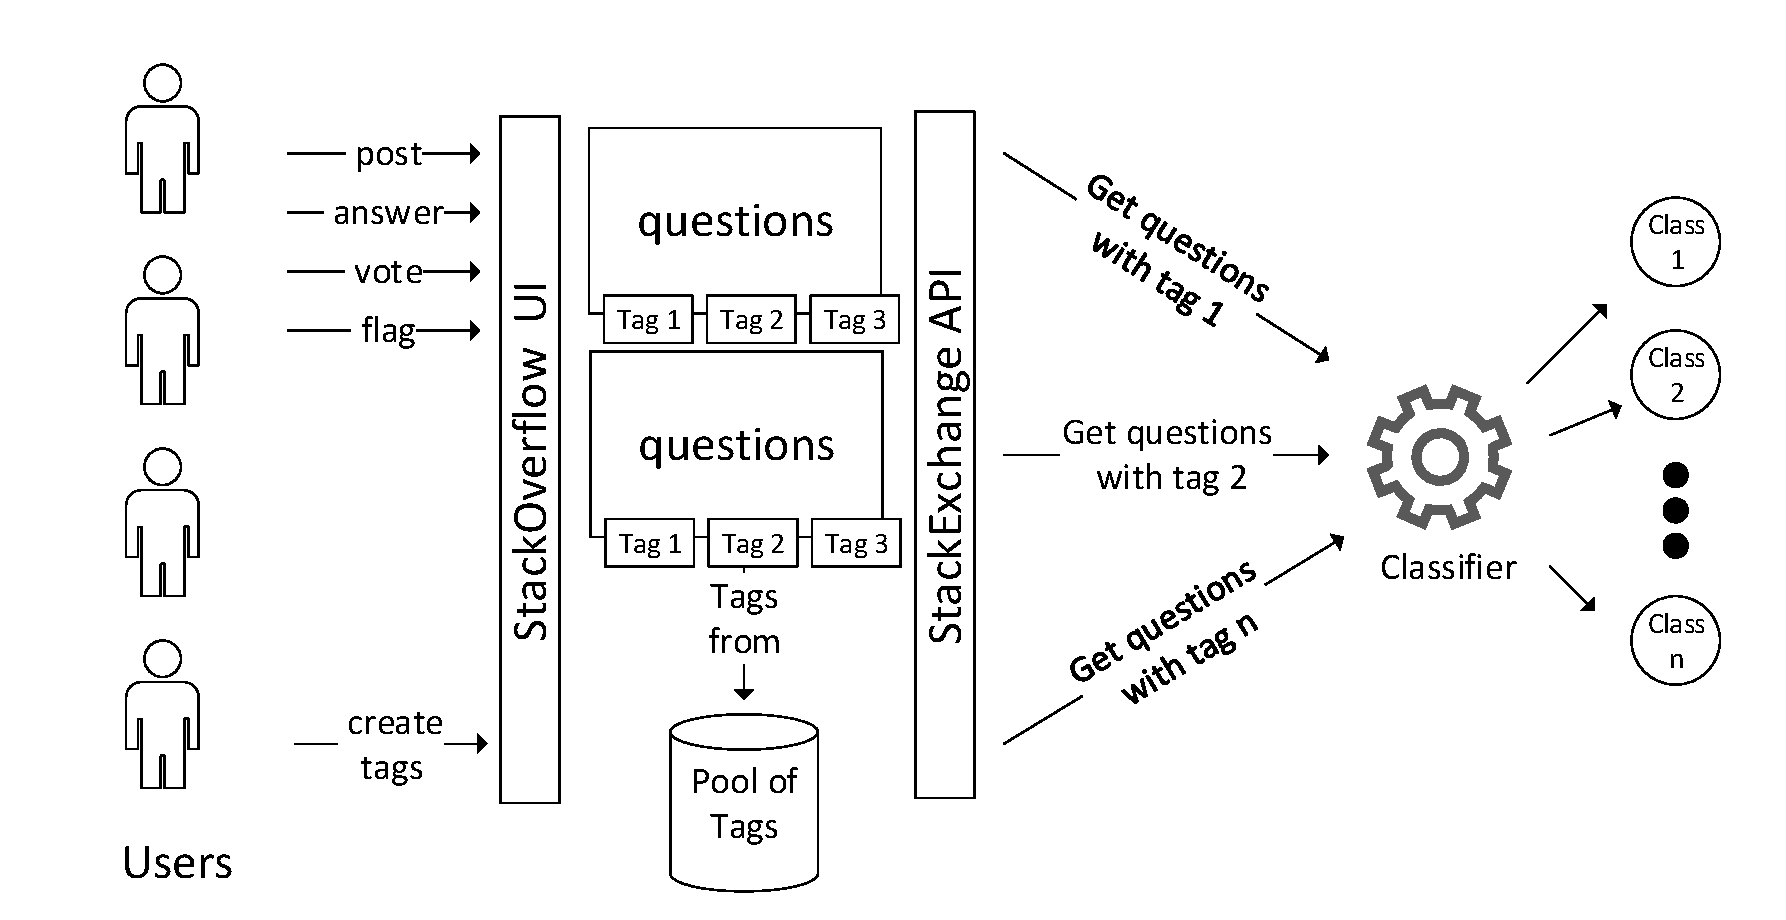
\includegraphics[width=1\textwidth]{./fig/StackOverFlow.pdf}
	\caption{The main StackOverflow users' actions and the topic classifier}
	\label{fig:stackoverflow_questions}
\end{figure}

The first training set of our Natural Processing Tool consisted of five tags, relative to our platform. Those tags were: \emph{scalability}, \emph{reliability}, \emph{design}, \emph{performance} and \emph{optimization} and we got thirty questions per tag. For each of the tags, the thirty most up-voted questions from StackOverflow were retrieved and classified to each specific tag. Those exact tags, after classification, are transformed in classes in NLP classification, as shows the Figure~\ref{fig:stackoverflow_questions}

Every time a user asks a question to one of the platform's communities, the classifier determines the class of the question. After the class is found, and if the platform is able to determine a heuristic answer, it will post then the answer to the user's question automatically. All the users of the platform can vote this answer up or down, depending on its accuracy, or provide their own answers.

The second training set of Natural Processing Tool was retrieved by automatically discovering tags. NB is trained with 10,000 questions from StackOverflow Q\&A site, fifty questions per each discovered tag. The general algorithm is shown below. Firstly, the algorithm starts with a tag that is relevant to the social network platform such as \emph{scalability} at line 01. Afterwards, using the SE API the algorithm gets the 5 most voted questions tagged with \emph{scalability}. For each question (line 04), the populateClassifier clears the body from any html tags inserted by the StackOverflow users to beatify their questions (line 05) and classifies this question's body with each tag. Automatically, the populateClassifier proceeds to the next tag of this question. When the populateClassifier is finished the NB is trained. It should be noted that a question may have more than one tags, so a question can be classified to up to five tags / classes. Changing the threshold parameter at the following algorithm, the \emph{populateClassifier} can classify questions with an arbitrary number of tags. At the following section the process to Bayes classification is described in more details.

\begin{lstlisting} 
01:var tags = ['scalability']
02:populateClassifier(0)
03:function populateClassifier(i) {
04:  var qs = stackexchange.api.getQuestionsByTag(tags[i])
05:  foreach(qs as q)
06:    body = clear(q.body)
07:    foreach(q.tags as t)
08:    	 classify(body, t)
09:    	 if(not tags.exist(t) and tags.length() < threshold)
10:    	   tags.push(t)	  
11:        populateClassifier(tags.indexOf(t))
12:}		
\end{lstlisting}

\subsection{Bayes classification algorithm}
This section describes the Bayes classification algorithm. As the above code snippet shows at line 08, the algorithm classifies a document named \emph{body} into the class \emph{t}. This \emph{body} is the content of the question that will be classified into the class \emph{t}, which is the tag of the question. Diving in this function, the \emph{body} is transformed to lower case and the Porter Stemming Algorithm~\citep{porter1980algorithm} is used for suffix stripping, so the plural form of the words and the suffixes are removed (such as \emph{-ing} and \emph{s}). For example, the following words: {\it connected}, {\it connection}, {\it connections}, {\it connecting}, {\it connectionless} will all be transformed to the single word ``connect''. The Porter Stemming Algorithm does not use any dictionary but a simple list of suffixes. This practise, makes the algorithm fast (10.000 different words in 8.1 seconds). After this process a table of words of this \emph{body} is kept.

After the populateClassifier has finished, the \emph{trainClassifier} is called (for simplicity the classifier is not shown in the above code snippet). The objective of \emph{trainClassifier} is to make the document body ready for Bayes Classification. The purpose of \emph{trainClassifier} is to count the number of occurrences of each word in each class.

After the above process is done, the classifier is ready, so when a future request for classification comes, the classifier returns the probability of a document being part of a class. This probability is calculated with the following formula:
\\
\[prob(d / c) = log\left ( \frac{countedTerms(d, c)}{totalsTerms(c)} \right )\]
\\
Where the probability of a document {\it d} to be in a class {\it c} is the logarithmic value of the division of the words(terms) of {\it d} found in class {\it c} by the total number of terms in {\it c}.

\subsection{Automated answers}
\label{sec:example_nlp}
As described in Section~\ref{sec:natural_implementation} Natural Language Processing is used to determine the users' input question in groups. 

When a user asks a question, the body of the question classified into categories and when the NLP classifies the question to a specific category, an approximate answer can be given in response. As the example shows in Figure~\ref{fig:nlp_example}, after the user's question, the classifier process the body and if the question is about the {\it JEnterprise} and the {\it cost effectivess} the approxiame answer ``The most cost effectiveness configuration of SPEC JEntreprise2010 is: jEnterprise18F \ldots'' is given. The users of the PaaSage social network platform can vote up or down the answer and/or provide their own answers.

\begin{figure}
  \centering
  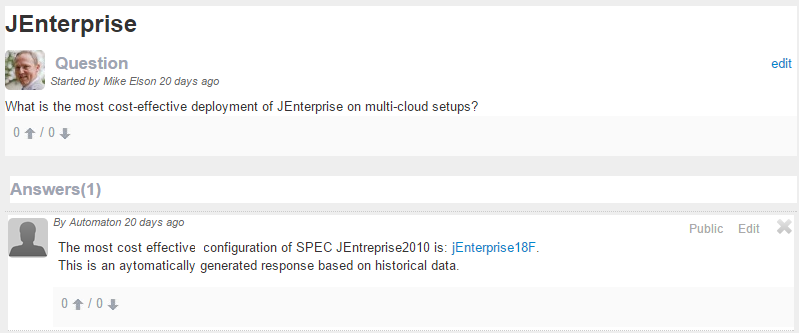
\includegraphics[scale=0.6]{./fig/nlp_example.png}
  \caption{Automated answer to user's question}
  \label{fig:nlp_example}
\end{figure}

The automated replies provide the user with a direct possible answer to the question. So, it reduces the time waiting for an answer and provides a first helping hint about the user's question. If the answer is not efficient, other potential user of SNP can provide answers to the question and down-vote the automated reply.

Finally, a relevant question can be asked to the platform as ``Which deployments of JEnterprise provide the best performance for the lowest cost in a multi-cloud setup?''. This question is a paraphrased question of the previous one, talking about the same thing. The platform can find this similarity and provide the same automated answer.

\section{User interface}
This part of the thesis describes the User Interface of the social network platform that is implemented based on 104 mock-ups created by HCI expert team. A mockup is a realistic representation of what the product will look like, in our case the social network platform. The design of look \& feel of SNP is made by HCI expert team in order to follow the modern trends in Web Applications design. In order to support those look \& feel and the functionality of those mock-ups 25K lines of php, js and css code is written.
The key design objective of the social network platform is to create a strong bond between (i) software engineering services for managing and deploying cloud-targeted application models; and (ii) community-oriented facilities for communication and
collaboration between users. The interconnections between the two in the design of the user interface are depicted in Figure \ref{fig:two_aspects}.
The prototype implementation is publicly accessible on-line at http://socialnetwork.paasage.eu. 

\begin{figure}[h]
	\centering
	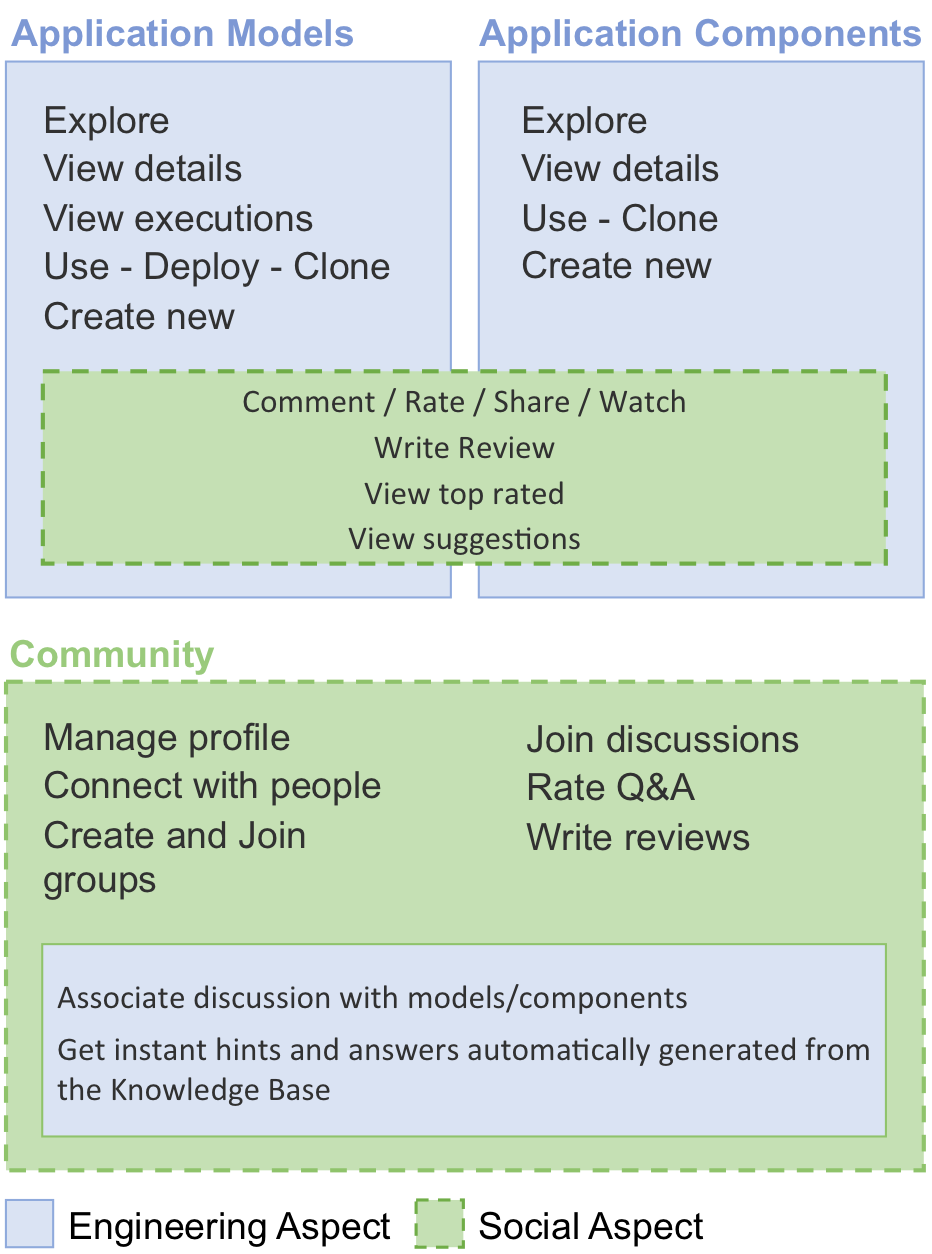
\includegraphics[width=0.6\textwidth,natwidth=200,natheight=150]{./fig/two_aspectes.png}
	\caption{Engineering and social activities are seamlessly interweaved within the social networking platform}
	\label{fig:two_aspects}
\end{figure}

\subsection{Design principles}
The discrete entities, which bind together the Social Networking with the application model aspects of platform are:
\begin{itemize}
\item \emph{Application Models}. Application Models is a key entity of the platform. An example is shown if Figure \ref{fig:jenter_home}, consisting of a human friendly description (label 1 in fig.\ref{fig:jenter_home}), the Camel Description of the model (label 2 in fig.\ref{fig:jenter_home}), reviews about the model (label 3 in fig.\ref{fig:jenter_home}). An overview of engineering aspects such as version and runs (label 4 in fig.\ref{fig:jenter_home}) and an overview of social aspects such as share and watch (label 5 in fig.\ref{fig:jenter_home}). The {\it share} action broadcast the model to the friends of the user that shares the model. The {\it watch} action notifies the user for future updates of the application model. 
\item \emph{Components}. We have integrated the Chef supermarket components into social network platform. The components help the DevOps users to generate their application models as described in~\ref{sec:automatedcreation}. 
\item \emph{Users}. Users who basically are cloud deployment specialists and other users who want to know which deployment configuration they should use. Users can exchange knowledge to groups and benefit from the CAMEL repository. They can create or join groups, ask and answer questions, follow application models and create their own network of friends.
\item \emph{Groups}. As mentioned, every user of PaaSage social network platform can create or join groups. Groups help users to interact with each other and gain knowledge from experts.
\end{itemize}

\begin{figure}[h]
	\centering
	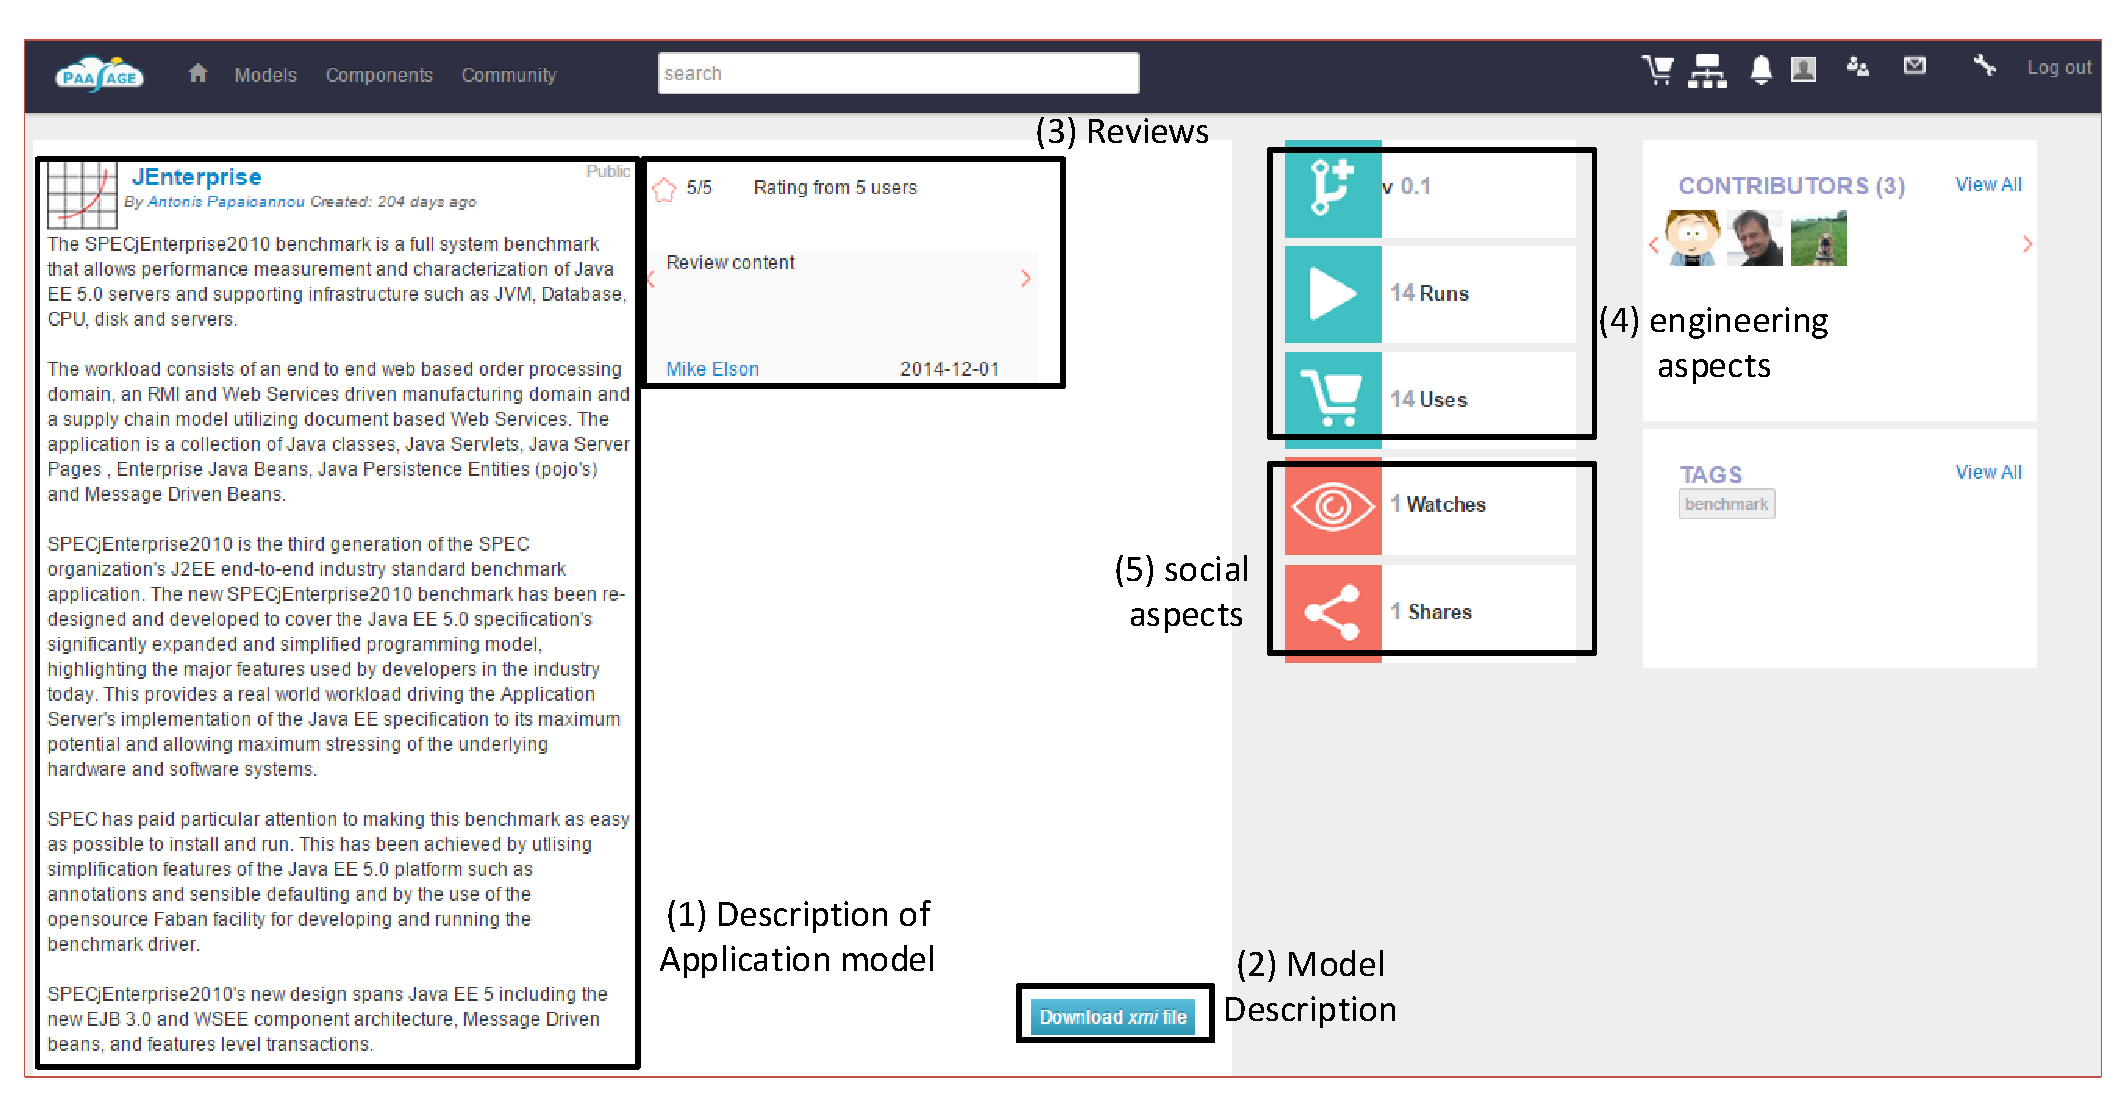
\includegraphics[width=1\textwidth,natwidth=200,natheight=150]{./fig/jenterprise_home_page.pdf}
	\caption{The application model home page}
	\label{fig:jenter_home}
\end{figure}

\subsubsection{Gamification}
Following recent trends in social networks design and with the aim to motivate users active and regular participation in
the professional network, the design employs gamification features, meaning the use of video game elements in order to improve user experience and user engagement in non-game services and applications~\cite{deterding2011gamification}. One gamification feature in the social network design is the reward system for active community members. As users contribute content (models, components, ratings, reviews, questions, or answers) they receive experience points leading to special badges visible to all community members. Other features are the Profile completeness bar with suggestions on how to increase it. Finally, the concept of Model badges awarded to application and component models in case of excelling performance. Badges can serve among others as goal-setting devices, status symbols, and indications of reputation assessment procedures~\cite{antin2011badges}.

\section{Generating application models}
The DevOps users of PaaSage social network platform can benefit from the automated creation of CAMEL baseline models presented at Section~\ref{sec:automatedcreation} or upload their own created models using external editors like EMF~\cite{cdomodel} tree based editor or GMF~\cite{gmf_url} editor presented at Section~\ref{sec:gmf}.

\subsection{Baseline models}
\label{sec:automatedcreation}
In order for users to create automated generated baseline CAMEL models, they can browse around the integrated Chef components inside the social networking platform and find the appropriate components for their applications. The platform has integrate a pointer for each Chef cookbook to the social network database using the Chef Supermarket API~\cite{chef_api_url}. A PHP command has implemented in order to iterated through all Chef cookbooks and update the repository of SNP. This command has been configured and runs one time every day.

Through the application model creation Page of the PaaSage social network platform, the users can upload an external CAMEL model description of their application or create a new one with the help of the platform in 4 simple steps as shown in Figure ~\ref{fig:model_creation_0}. In the step zero~\ref{fig:sfig0}, the user is asked whether the new Application model already has an CAMEL model or whether the user wants to create a new application CAMEL model through automated generation. For automated generation, the user must previously put the Chef cookbooks that he/she wants in the user's cart. The selected Chef cookbooks will be shown as a list of components. Then, in step one~\ref{fig:sfig1}, the user selects from this list which of the components will be included in the application model. 
In the example shown, the user has four components {\it mysqld}, {\it apache2}, {\it nodejs} and 
{\it ruby\_installer} and selects three of them. In the next step, shown in Figure~\ref{fig:sfig2}, the user provides the deployment information (to which cloud provider the Application will run and which type of VMs will be used). Also, some components can be collocated in the same VM. In this example, the {\it nodejs} component will be collocated in the same VM as the {\it apache2}. In step tree, shown in Figure~\ref{fig:sfig3}, the user provides the communication information between the components, for example the 
{\it nodejs} communicates with {\it mysqld} in the default mysql port {\it 3306}.

In the final step as shown in Figure~\ref{fig:sfig4}, the user provides the final needed information about the name of the Application model, a human friendly description and the version of the model. In the bottom of the form of the Figure~\ref{fig:sfig4} the user can find three actions: the \emph{Previous} action, the \emph{Save as draft} action and the \emph{Finalize} action. The \emph{Previous} action can performed all around the steps and make the user easily walk around the steps, giving him/her the opportunity to alter an option. The \emph{Save as draft} action creates the CAMEL model of the application but the model is not publicly available and only the creator or the contributors of the Application can see or edit the Model. The \emph{Finalize} action creates the CAMEL model of the application and makes it publicly available to the SNP users. 

For the creation of the base line CAMEL model an AJAX request is sent to a Java tool, that automatically creates the application model according to the information that the user has already provided. When the Java tool generates the CAMEL model, it sends it back to the SNP. So the SNP can store this model to the repository. This tool is presented at~\cite{papoutsakis2014reducing}. 

\begin{figure}
\begin{subfigure}{.8\textwidth}
  \centering
  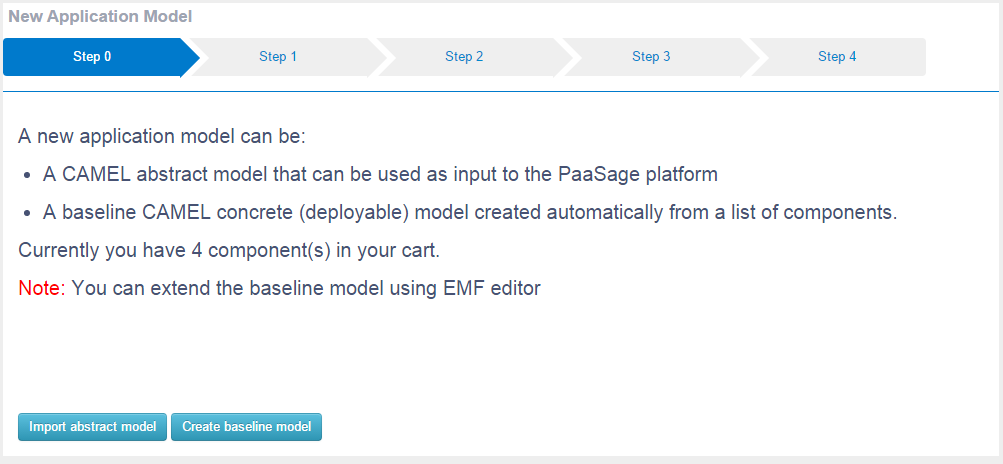
\includegraphics[scale=0.4]{./fig/model_creation0.png}
  \caption{Step 0: Upload external or create baseline model}
  \label{fig:sfig0}
\end{subfigure} \\[1ex]
\begin{subfigure}{.8\textwidth}
  \centering
  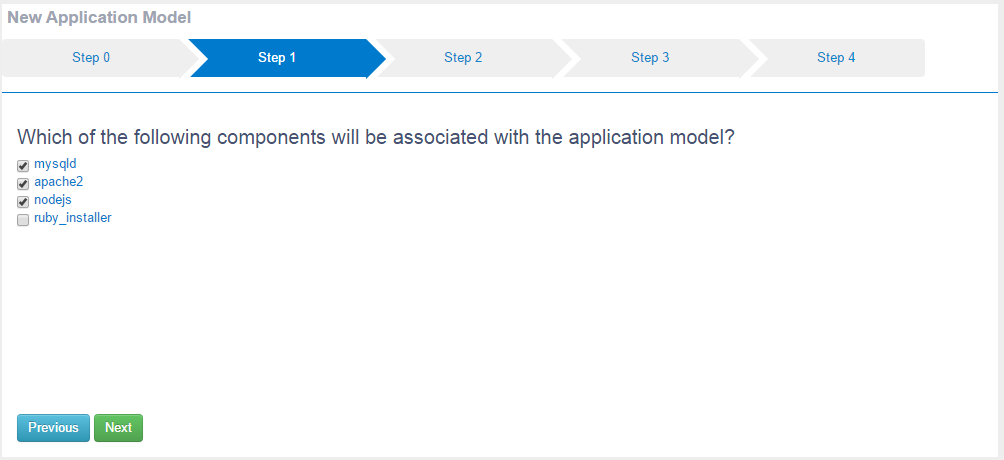
\includegraphics[scale=0.4]{./fig/model_creation1.png}
  \caption{Step 1: Choose the components from the users' list}
  \label{fig:sfig1}
\end{subfigure} \\[1ex]
\begin{subfigure}{.8\textwidth}
  \centering
  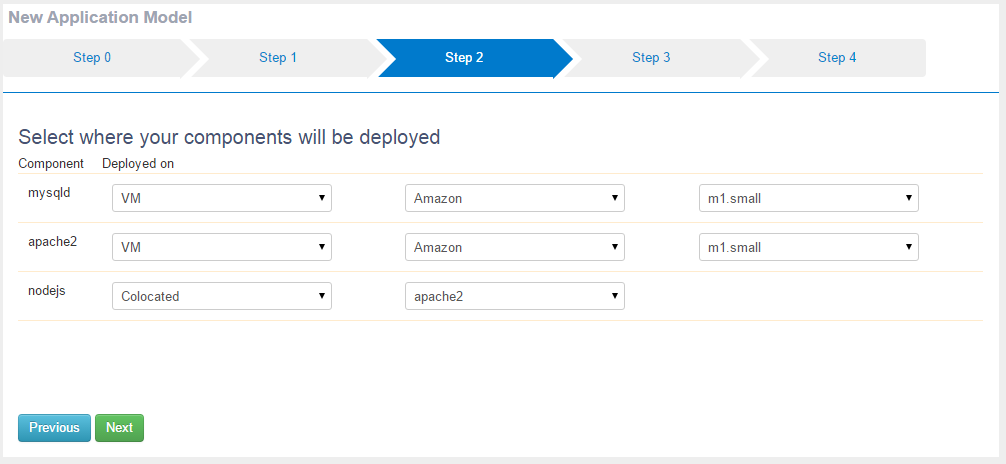
\includegraphics[scale=0.4]{./fig/model_creation2.png}
  \caption{Step 2: Deployment information}
  \label{fig:sfig2}
\end{subfigure} \\[1ex]
\begin{subfigure}{.8\textwidth}
  \centering
  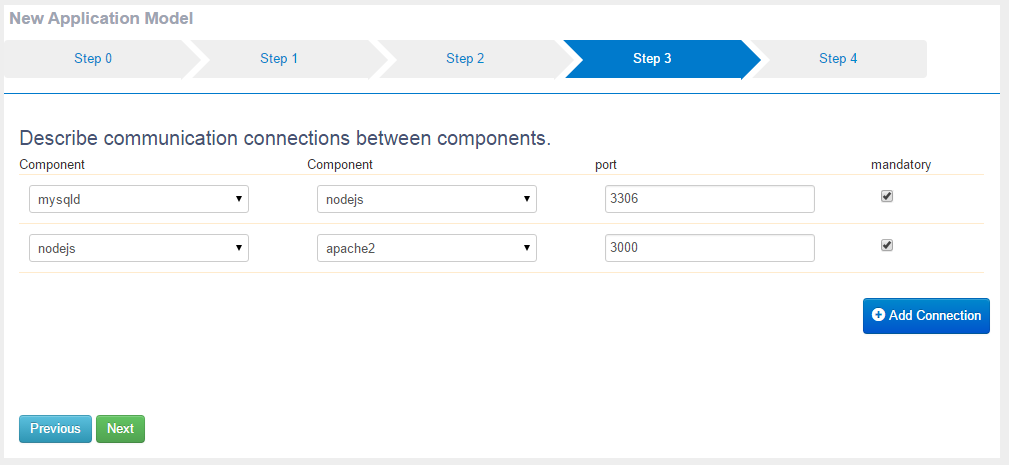
\includegraphics[scale=0.4]{./fig/model_creation3.png}
  \caption{Step 3: Communication information}
  \label{fig:sfig3}
\end{subfigure} \\[1ex]
\caption{Steps for automated creation of baseline model}
\label{fig:model_creation_0}
\end{figure}

\begin{figure}
  \centering
  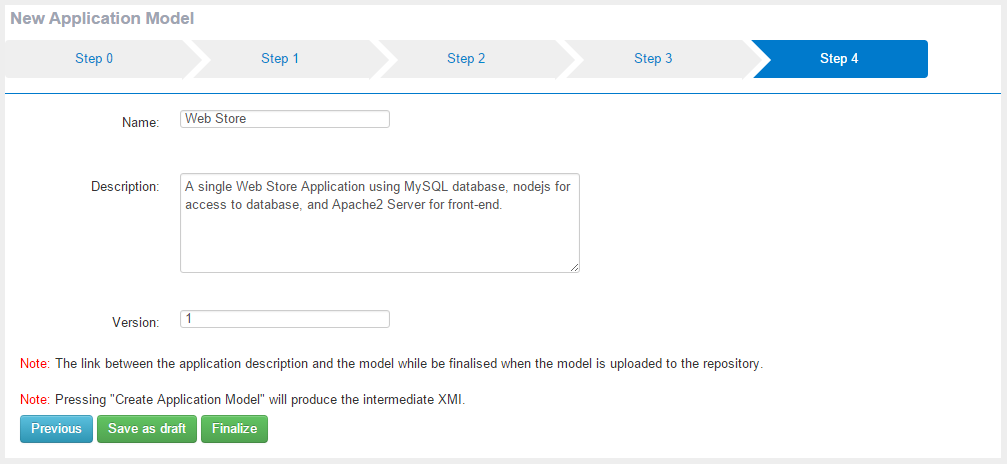
\includegraphics[scale=0.4]{./fig/model_creation4.png}
  \caption{Final step of automated creation of baseline model.}
  \label{fig:sfig4}
\end{figure}

\clearpage

\subsection{Graphical modeling}
\label{sec:gmf}
Advanced users of the PaaSage social network platform can compose application models through Graphical Modeling Framework (GMF)~\cite{gmf_url} which is an external Eclipse editor. GMF provides a set of generative components and runtime infrastructures for developing graphical editors based on Eclipse Modeling Framework (EMF) and Graphical Editing Framework (GEF). The GMF editor is generated from CAMEL {\em ecore} schema and provides the graphical palette to compose applications. 

Figure~\ref{fig:sensapp_as_gmf} shows the composition of a sample application model with the GMF editor. The palette in the right, contains all nodes and relationships needed to describe an application model. In the center, the composition of a sample application is shown, consisting of three VM types, the VM information about these VMs and the owner/user of the application. The GMF editor generates two files, one responsible for the graphical representation and the XMI description of the application model that can be uploaded to the social networking platform.

\begin{figure}
  \centering
  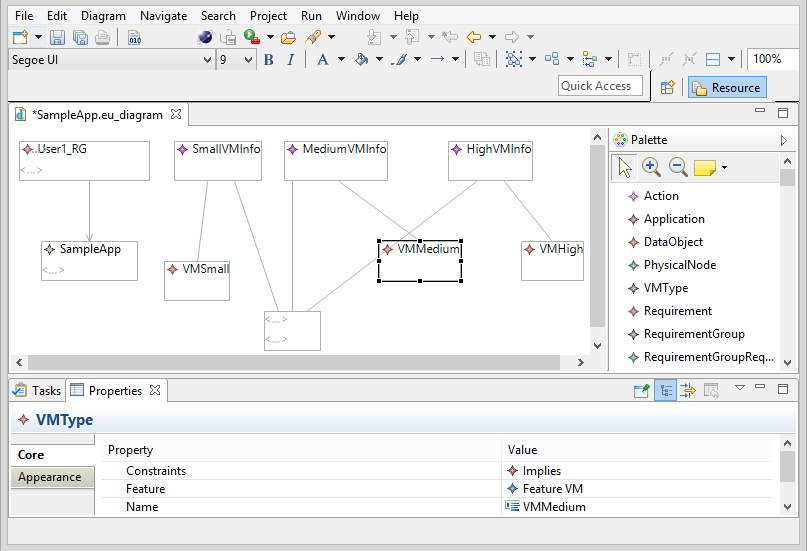
\includegraphics[scale=0.6]{./fig/gmf_editor.png}
  \caption{GMF editor composition of a sample application}
  \label{fig:sensapp_as_gmf}
\end{figure}

\chapter{Evaluation}
\label{chapt:evaluation}
This Chapter describes the evaluation of the scalability of the system architecture, the evaluation of the topic classification mechanism and the collaboration and contribution to user interface evaluation.  

\section{Scalability}
\label{sec:eval_scalability}
This Section describes the evaluation of the two different implementations of the system architecture. In the first architecture, more than one memcached instances at layer 2 were introduced, as Figure~\ref{fig:system_architecture} shows. In the second, more than one Social Network engines were introduced at layer 1.

In order to measure the response time (RT) the Apache JMeter application~\cite{jmeter_url} is used. The Apache JMeter is an open source benchmark designed to test functional behaviour and  measure performance, targeting web applications. Notably, the RT measured by JMeter may not be the real one, because the JMeter measures the elapsed time from just before sending the request to just after the last response from the server has been received. As a result, the time to render the web page to the client web browser and the execution time of JavaScript code is not measured. Because those two time intervals are client limited and depend on client performance and on which web browser is used, they are excluded from the following performance test benches. For the next experiments, a specific web page will be used. This page does not use any AJAX call, in order to not misguide the results. Therefore, the RT measures the time from just before JMeter sends the request to just after the last response is received. During this measured time interval, the Social Network engine performs the following actions:
\begin{enumerate}[I]
\item The Social Network engine sends a request to CDO Client for the application execution model.
\item The CDO Client forwards this request to CDO Server.
\item Afterwards CDO Server queries the mysql repository of application models and executions, and finally gets the executions results.
\item CDO Server forwards the results through the CDO Client to the Social Network Engine.
\item Finally, the Social Network engine sends queries to the Social Network DB in order to get all the necessary Social features for this application page
\end{enumerate}

The presented system architecture was deployed on Amazon EC2~\cite{amazon_url} and the system CPU Utilization and the response time of SNP is measured.

\subsection{Focusing on memcached}
\label{sec:eval_memcache}
By adding a Memcached node at the system architecture, the Social Network Engine first asks the Memcached node if it has the tuples that the SN Engine needs. So the steps(\emph{I} to \emph{V}), mentioned previously, are not necessary if the Memcached node has cached the values that the Social Network Engine needs. The loop through CDO CIient - CDO Server and the repositories is bypassed. 

\begin{table}[]
\centering
\caption{Number of Queries from Social Network and CDO server repository.}
\label{tab:num_of_queries}
\begin{tabular}{ll}
State        & \# of Queries \\
Fresh start  & 1938          \\
Fresh Query  & 15182         \\
Cached Query from CDO & 251           \\
Cached Query from Memcached & 147  
\end{tabular}
\end{table} 

For the following experiments all the Memcached nodes are warmed up and have already cached all the needed CDO and Social entities information. Furthermore the CDO server has been warmed up after a fresh restart. As the Table~\ref{tab:num_of_queries} shows,
the starting process of the CDO server produces 1938 queries to MySQL database. The \emph{fresh query} for an application model (both social information and executions) produces 15182 queries to MySQL database. The CDO server caches the results, so a second query for this application model produces 251 queries, most of which are the queries for the social information of the application. Introducing Memcached, if the request for the application model is cached, the queries to database are lowering to 147.  

\begin{figure}[h]
	\caption{The average response time for all configurations.}
	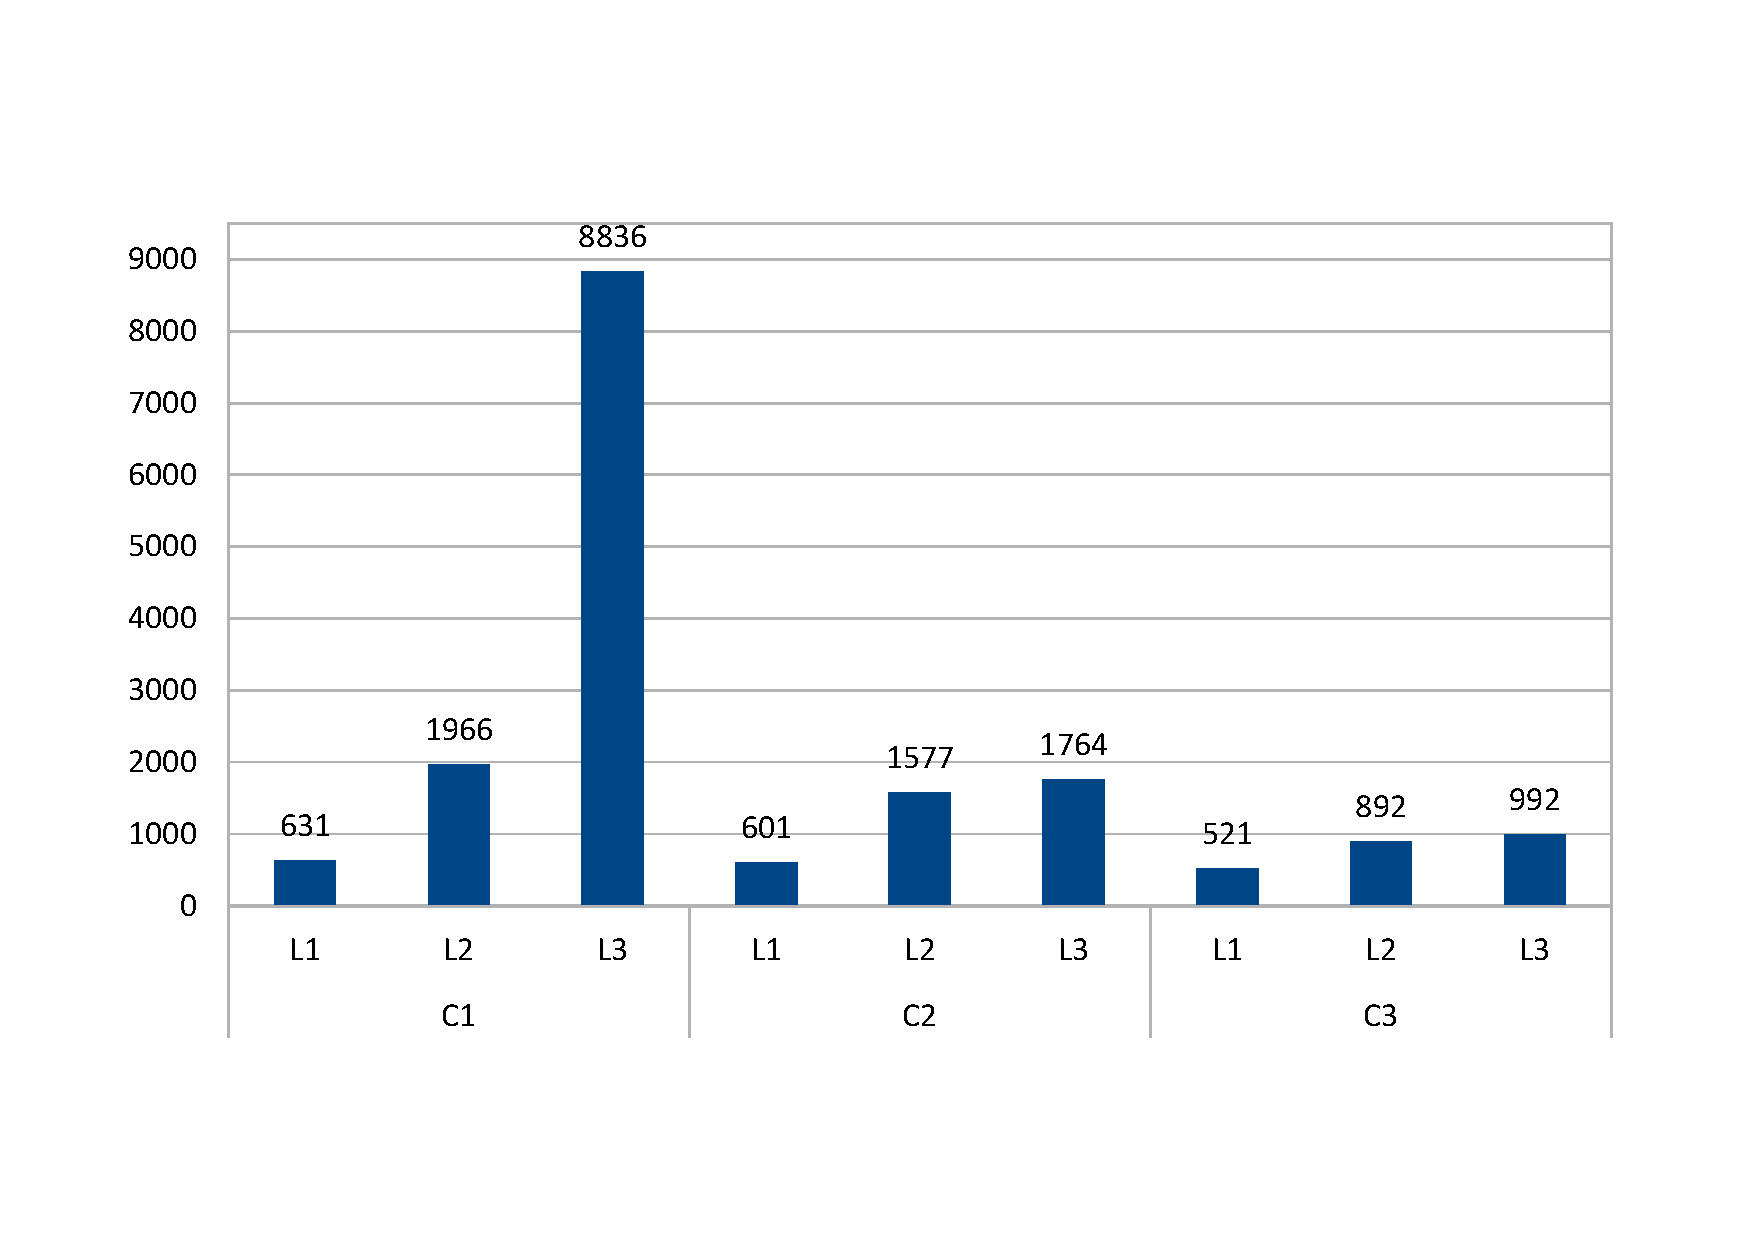
\includegraphics[width=0.9\textwidth,natwidth=200,natheight=150]{./fig/RTavg.pdf}
	\centering
	\label{fig:rtavg}
\end{figure}

The test performed with the following loads: (L1) ten users request \emph{two} applications, (L2) ten users request \emph{four} applications and (L3) ten users request \emph{eight} applications. All three Loads run consecutively one hundred times each. Those Loads request applications, which have ten execution rows pulled from the repository of applications models and executions, and about one hundred queries to the Social Network DB. In this experiment we kept the following components of the system constant: the Elgg front-end Apache2 server, the Social Network Database, and the CDO server - client communication but we increased the number of Memcached nodes.
The Figure~\ref{fig:rtavg} shows the  average response time (RT) in milliseconds with the following system configuration(C): (C1) no Memcached node , (C2) one Memcached node and (C3) two Memcached nodes have added to the system architecture.

As we going from C1 to C3 and specifically for L3, the RT is reduced by 80,4\% at C2 and by 88,78\% at C3. As the Figure~\ref{fig:rtavg} shows, at the first configuration C1, the L3 takes 8836 ms, an RT which is definitely prohibitive for web applications. Introducing more Memcached nodes at C2 and C3 the RT is decreased dramatically at 1764 ms at L2 and at 992 ms at L3. Going from C1 to C2, the 80,4\% reduction of RT is due to the introduction of Memcached node and bypassed the steps I - V. Going from C2 to C3, the 43,77\% reduction of RT. The reduction of RT is achieved by adding more Memcached nodes, which results to more CPU cores introduced to the architecture as described below.

\begin{figure}[h]
	\caption{The average CPU utilization for all components.}
	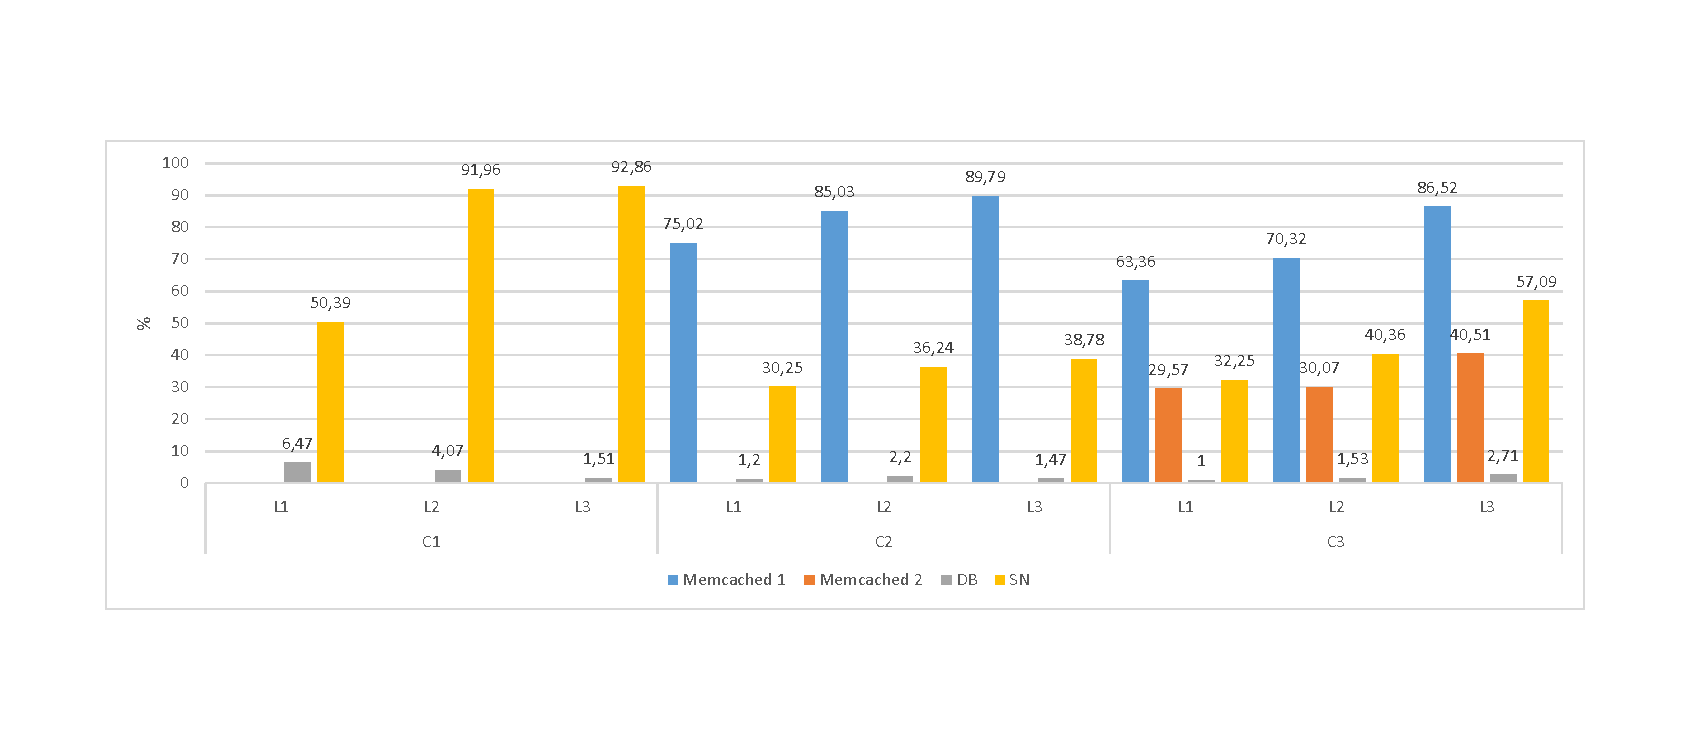
\includegraphics[width=1.1\textwidth,natwidth=200,natheight=250]{./fig/UsageAVG.pdf} 
	\centering
	\label{fig:cpuavg}
\end{figure}

The CPU utilization is measured using the sysstat tool~\cite{sysstat_url}. We measured the CPU utilization for all the VMs running the experiment. The information about the VM resources is listed in the Table~\ref{vms_resources}. The Social Network Engine and the CDO Client were running at t1.micro instance. The mysql (repositories) and the CDO Server were running at m1.xlarge. The average CPU utilization is shown in the Figure~\ref{fig:cpuavg}. At the simple configuration C1, even in small loads such as L1, the SN Engine reached 50,39\% CPU utilization. In the medium load L2 and big load L3 the SN Engine is kneeled down to 91,96\% and 92,86\%. This big consumption of CPU was due to all the initialization that Elgg Social Network Engine has to do for each request and due to CDO Server queries.

Moving from configuration C1 to C2, the CPU consumption went to Memcached node. Thus, the Social Network engine was de-congested and the RT improved. However, for the big load L3 the Memcached node reached 89,79\%. To solve Memcached CPU overhead, one more Memcached node was added at configuration C3. This second Memcached node shared the CPU overhead with the first Memcached node and the RT improved furthermore. 

For all three loads at C3, the first Memcached node had more CPU utilization from the second by an approximately factor of 2,2. This difference between the two Memcached nodes appeared due to the first node storing more popular key-value pairs than the other.

\begin{table}[]
\centering
\caption{VM resources. }
\label{vms_resources}
\begin{tabular}{|l|l|}
\hline
 Component &  VM type \\ \hline
 SN engine, CDO client &  t1.micro \\ \hline
 memcached &  t1.micro \\ \hline
 repositories, CDO Server &  m1.xlarge \\ \hline
 jmeter &  m1.large \\ \hline
\end{tabular}
\end{table}

\subsection{Focusing on the Elgg engine}

\begin{figure}[h]
	\caption{The Response time for two Social Network Engines.}
	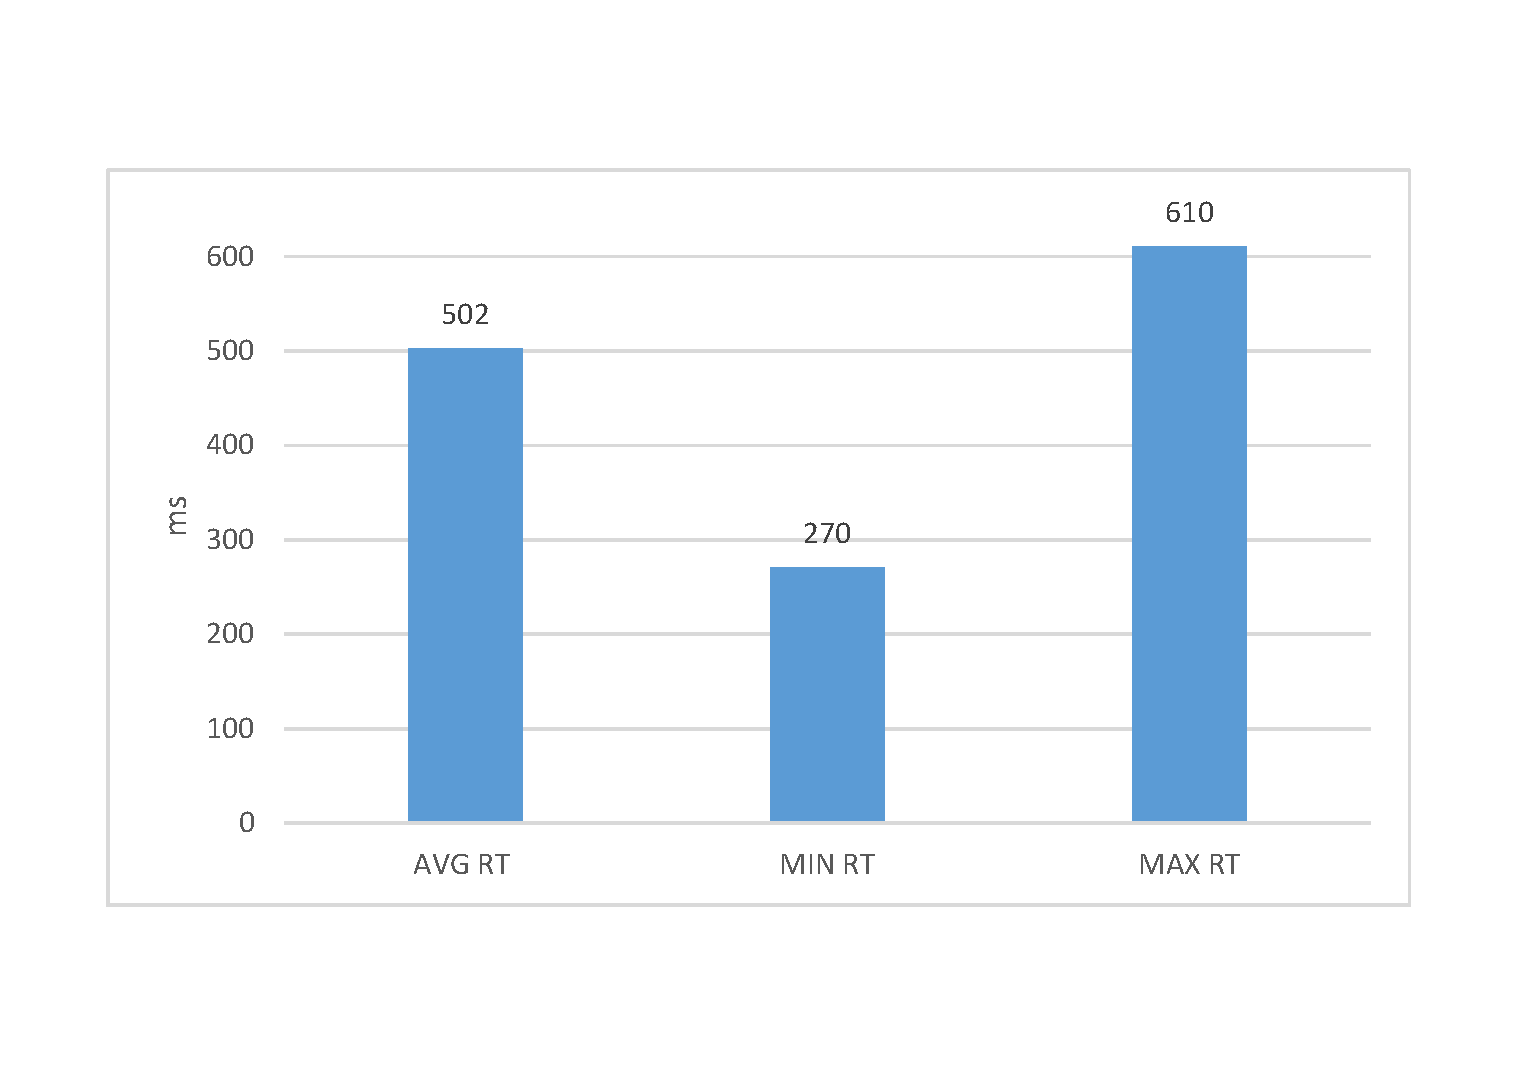
\includegraphics[width=0.8\textwidth,natwidth=200,natheight=150]{./fig/RT2SN.pdf}
	\centering
	\label{fig:rt2SN}
\end{figure}

\begin{figure}[h]
	\caption{The CPU utilization for two Social Network Engines.}
	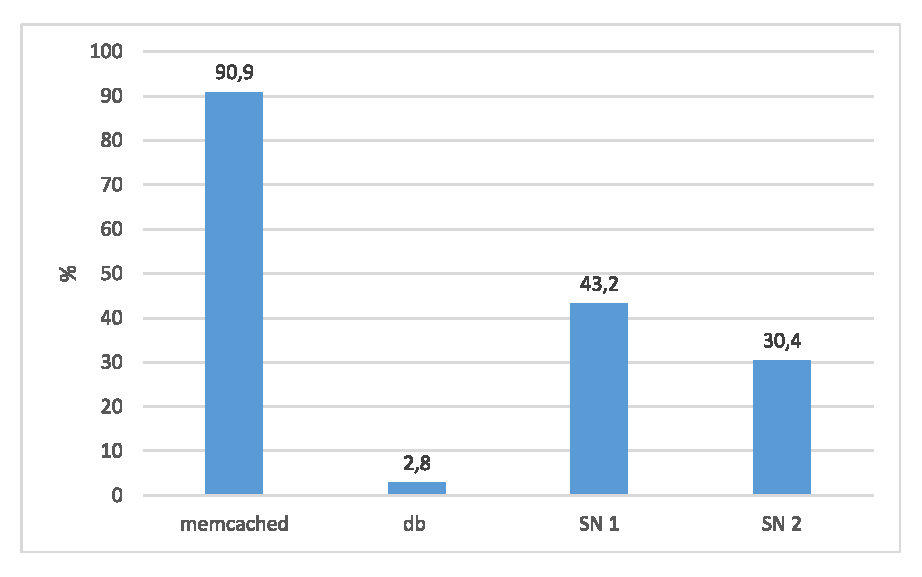
\includegraphics[width=0.8\textwidth,natwidth=200,natheight=150]{./fig/Usage2SN.pdf}
	\centering
	\label{fig:cpu2SNavg}
\end{figure}

This Section evaluates the horizontal scale of Social Network engine as described in~\ref{sec:engine_scale}. A memcached node was living between the Social Networking Engines and the back end system. The VM resources were kept the same as in the previous experiment and shown in the Table~\ref{vms_resources}. One more Social Networking Engine instance was added with the same type as former SN Engine. 

So, the system architecture now consists of two Social Networking Engines as front-end. At the back-end of the system we have: (1) one Memcached node and (2) the CDO client - server, the Social Network Database and the CDO repocitory. The two SN Engines are deployed to a dedicated VM each. Furthermore, each SN Engine has its own CDO client deployed with them. The Memcached node is deployed on its own VM and the CDO Server, the Social Network Database and the CDO repository are deployed on the same VM.

The Figure~\ref{fig:cpu2SNavg} shows the average CPU utilization for the Memcached, the MySql Database (db) and the two SN Engines (SN1, SN2). The load for this experiment is the same as the previous L3, which means we have ten users that request \emph{eight} applications for one hundred times consecutively. The first SN Engine has 43,2\% CPU usage and the second one has 12,8\% less. This difference is due to the first instance being deployed together with the NFS server and Apache Zookeeper on the same VM. 

With only one SN Engine the CPU Utilization was 57,09\% and now with two SN Engines the CPU Utilization is reduced to 43,2\%. This reduction is due to the requests being distributed to two instances instead of the only one instance. The CPU Utilization of the Memcached node increased, but this can be solved by introducing more Memcached nodes as the previous Section describes. Furthermore, we can introduce more SN Engines to support more heavy loads.

Since, the load from one SN Engine is now distributed to two SN Engines instances, the response time improved for the Load 3, as shown in the Figure~\ref{fig:rt2SN} compared to the previous test-bench. The best achieved RT of previous architecture was 992 ms and with this architecture it reduced to 502 ms.

We can combine the two architectures together, meaning that we have more than one SN Engine and more than one Memcached to support as many loads as we want.

\section{Topic classification}
\label{sec:nlp_evaluation}
This Section evaluates the topic classification tool as described in Section~\ref{sec:natural_implementation} for the first training set. This set had five different classes or, according to StackOverflow dialect, five tags, as described in~\ref{sec:natural_implementation} and shown in Table~\ref{table:nlp_eval}. For the testing set, thirty questions from StackOverflow were used per class. Those questions were different from the training set and had the highest activity during that specific time period. Each row at Table~\ref{table:nlp_eval} shows a class as classified by StackOverflow users, and each column shows how our classifier classifies the question. For example, twenty one questions about \emph{reliability} were classified correctly, but eight were wrongly classified as \emph{optimization} and one was wrongly classified as \emph{performance}. The misclassification however, was not an error of our classifier. The reason of these mistakes is that  some questions from the testing set were either wrongly classified by the StackOverflow users or had more than one tags. For example, one question that was wrongly classified as \emph{performance} instead of \emph{reliability} was: ``can somebody explain me how to handle errors. my code is: \ldots''. The above question is out of the scope of reliability and even though the user tagged it as a reliability question, it was downvoted and marked as ``very low quality'' from the StackOverflow community.

Another example showing that the classifier is not misclassifying, but the problem stands in the users' tagging, is the following question:
``I want to perform some data manipulation tasks and analysis in spark and want to \textbf{optimize} the run times. 
here is the problem: \ldots ''. 
This question was marked by the user with both scalability and optimization tags. Even though this question is retrieved with the scalability tag and in the Table~\ref{table:nlp_eval} it is shown as a wrong classification, after examining this question, one can realize that the \emph{scalability} tag was wrongly added by the user and only the \emph{optimization} tag should be placed.

This shows that our tool can further be used by StackOverflow to mark new questions that are wrongly tagged or misguided. There is a trend among StackOverflow users to add as many tags as they can in order to attract the attention of other users, increase the views of their question and finally get their answers.  

The true positive, which means a document is recognized in the correct class, according the Table~\ref{table:nlp_eval} is 85. The false positive, which means a document is not correctly recognized, of this topic evaluation is 65. According to those precision metrics the accuracy or sensitivity of our topic classifier for this specific experiment is 56,67\%.

\begin{table}[]
\centering
\caption{NLP Evaluation of Classification}
\label{table:nlp_eval}
\begin{tabular}{|l|c|c|c|c|c|}
\hline
class / class & \multicolumn{1}{l|}{reliability} & \multicolumn{1}{l|}{design} & \multicolumn{1}{l|}{optimization} & \multicolumn{1}{l|}{performance} & \multicolumn{1}{l|}{scalability} \\ \hline
reliability   & \textbf{21}                    & 0                           & 8                                 & 1                                & 0                                \\ \hline
design        & 2                                & \textbf{17}               & 6                                 & 3                                & 2                                \\ \hline
optimization  & 2                                & 3                           & \textbf{16}                     & 8 & 1                                \\ \hline
performance   & 1                                & 1                           & 11                                & \textbf{16}                     & 1                                \\ \hline
scalability   & 6                               & 3                           & 3                                 & 3                                & \textbf{15}                     \\ \hline
\end{tabular}
\end{table}

\section{Requirements and user interface}
\label{eval_ui}
The User Interface of social networking platform is designed through the iterative process of several expert-based evaluations being carried out in group sessions. To obtain additional feedback from non-experts, three additional user-based evaluation experiments were designed and carried out involving potential users and presented in~\cite{magoutis2015design}. 

The author collaborated in the expert-based evaluations sessions focusing on the platform user interface design. Furthermore, the contributions of the author, in the user interface evaluations, was to make the platform support them and also author took part in the third evaluation process.  

The first experiment, carried out by Flexiant Ltd. aimed at assessing the overall look and feel of the network, the navigation mechanisms, as well as the design of fundamental functionality.

The second evaluation experiment, carried out by HCI team, aimed to collect subjective results rather than performance metrics. It involved another set of 12 users who, after a brief introduction to the available facilities, were asked to use the interactive prototype~\cite{Virzi1996} using the free exploration method of the Thinking Aloud protocol~\cite{jordan1998introduction} and fill-in a questionnaire in order to rate and comment their experience. 

The third evaluation experiment involved 15 participants who were guided through the interactive prototype of the PaaSage social network using specific scenarios. They were interviewed on their requirements and feedback following a semi-structured interview approach [84]. The evaluation session was carried out via Skype. Participants were recruited through European companies and organizations associated with the PaaSage EU project~\cite{paasage}. They were either developers or operations staff, thus within the target user groups of the PaaSage social network. Participants were not users of the PaaSage platform; some however were familiar with the project’s goals and objectives. Before the experiment, each participant was requested to fill-in a background information form and was sent an informed consent form, explaining all the recording and anonymity-ensuring procedures. 

\begin{figure}[h]
	\caption{SNP features that were mostly liked by the users.}
	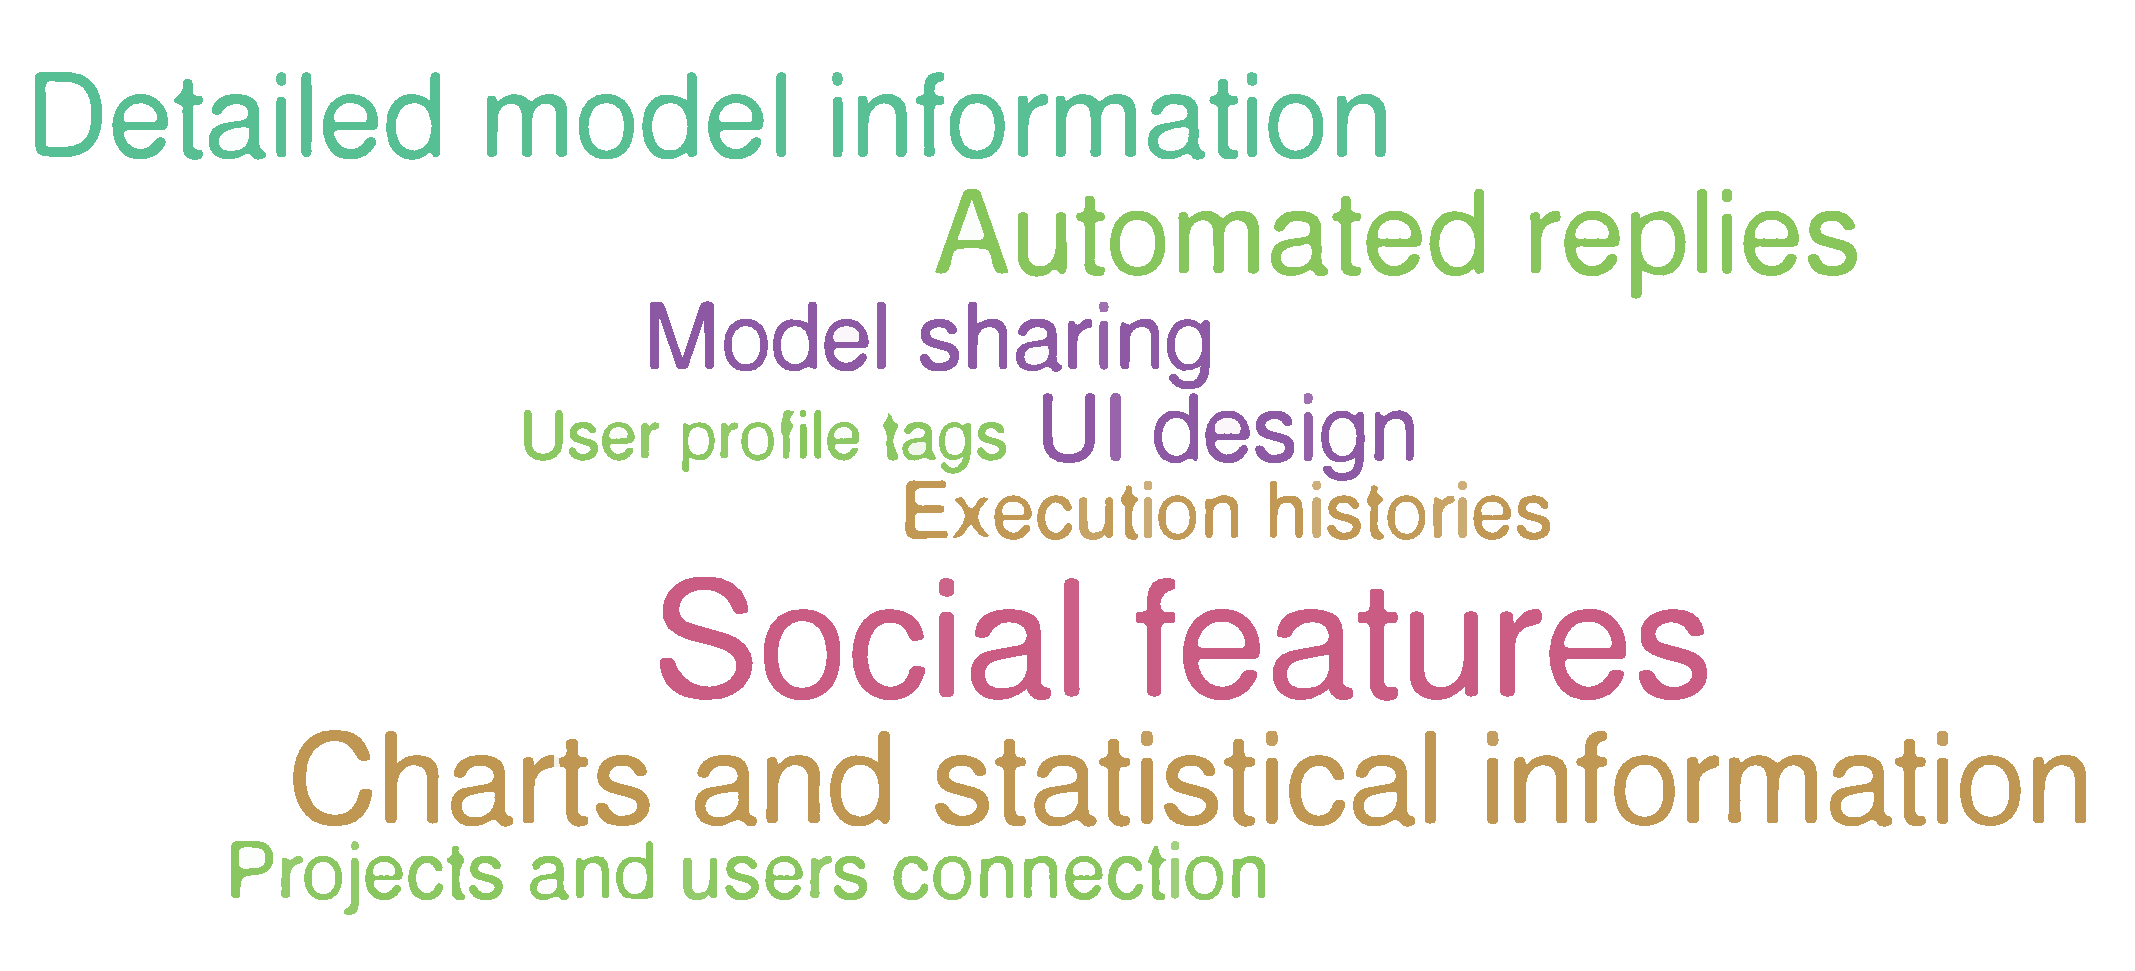
\includegraphics[width=1\textwidth,natwidth=200,natheight=150]{./fig/most-liked.pdf}
	\centering
	\label{fig:most-liked}
\end{figure}

Users, in the third experiment, were asked to identify up to three most-liked and three most-disliked features. Most-liked features presented in Figure~\ref{fig:most-liked} included: the employment of social features in a development environment; the use of charts and statistical information to represent data; the detailed model information that could be retrieved and the model execution histories; the automatically-generated hints provided by the network as replies in discussion topics; the concept of sharing one’s models; the overall UI design; the direct connection between projects and users, and the user profile tags that allowed them to find users that would be interesting to connect with.

Those evaluation experiments show that a platform that couples together the employment of social networking features in community-building activities with the DevOps demands about application deployment, the execution analysis, the automatically generated hints based on data analysis is a helpful tool that people would like to use.
%\chapter{Comparison}

Compare your work \ldots

\section{AA}
\section{BB}

\chapter{Conclusions and Future Work}
In this thesis a scalable Social Network for DevOps users is presented. The scalining of the system presented at the front end layer by introducing more than one Social Networking Engine instances, or at the back end of the system by introducing more than one memcached nodes. The DevOps users of the Social Network can benefit from the \ldots
\bibliographystyle{IEEEtran}
\bibliography{references}

\end{document}
